\documentclass[xcolor=table,fleqn]{beamer}

\usetheme[secheader,compress]{Madrid} %Primary theme
\setbeamertemplate{headline}{}  % uncomment this line if do not want headline shown in every frame.

% Change base colour beamer@blendedblue (originally RGB: 0.2,0.2,0.7)
%\colorlet{beamer@blendedblue}{red!40!black}  % For College of Charleston (Maroon and White)

\setbeamertemplate{navigation symbols}{}
\setbeamertemplate{bibliography item}{\insertbiblabel}

\usepackage{xcolor}
\usepackage{epsfig}
\usepackage{stackengine}
\usepackage{hyperref}
\usepackage{multirow}
\usepackage{graphicx}
\usepackage{amsfonts}
\usepackage{array}
\usepackage{ulem}
\usepackage{amsthm}
\usepackage{textpos}
\usepackage{subcaption}
\usepackage{graphicx}
\usepackage{pbox}
\usepackage{tikz}
\usetikzlibrary{shapes}
\usepackage{tabularx}
\usepackage{framed}
\usetikzlibrary{arrows}
\usepackage{amsmath}
\usepackage{datetime}
\usepackage{savefnmark}
\usepackage{transparent}

%%%%%% Comment the following two if want bib info display in later frames.
\usepackage[backend=bibtex]{biblatex}
\bibliography{research}
%%%%%%

\usepackage{bibentry}
\usepackage{chngcntr}
%\counterwithin*{footnote}{page}
\newcommand{\footcitefull}[1]{%
    \addtocounter{footnote}{1}%
    \footnotetext[\thefootnote]{%
        \addtocounter{footnote}{-1}%
        \refstepcounter{footnote}\label{#1}%
        \fullcite{#1}%
    }%
    $^{\ref{#1}}$%
}
\newcommand\secondcite[1]{$^{\ref{#1}}$}

\tikzset{
  main node/.style={circle,draw,font=\small},
  rectangle/.style={font=\small},
	empty/.style={edge from parent/.style={}}
}

\setlength{\mathindent}{0pt}

\makeatletter
\newcommand{\removelatexerror}{\let\@latex@error\@gobble}
\makeatother

\makeatletter
\def\dual#1{\expandafter\dual@aux#1\@nil}
\def\dual@aux#1/#2\@nil{\begin{tabular}[b]{@{}c@{}}#1\\#2\end{tabular}}
\makeatother

\let\proof\relax
\let\endproof\relax

\setbeamercolor*{bibliography entry title}{fg=black}
\setbeamercolor*{bibliography entry author}{fg=black}
\setbeamercolor*{bibliography entry location}{fg=black}
\setbeamercolor*{bibliography entry note}{fg=black}
\setbeamertemplate{bibliography item}{}

\newcounter{saveenumi}
\newcommand{\seti}{\setcounter{saveenumi}{\value{enumi}}}
\newcommand{\conti}{\setcounter{enumi}{\value{saveenumi}}}

%%% Customize the footline of the title page
\makeatletter
\setbeamertemplate{footline}
{
  \leavevmode%
  \hbox{%
  \begin{beamercolorbox}[wd=.333333\paperwidth,ht=2.25ex,dp=1ex,center]{author in head/foot}%
    \usebeamerfont{author in head/foot}\insertshorttitle
									 %\beamer@ifempty{\insertshortinstitute}{}{(\insertshortinstitute)}
  \end{beamercolorbox}%
  \begin{beamercolorbox}[wd=.333333\paperwidth,ht=2.25ex,dp=1ex,center]{title in head/foot}%
    \usebeamerfont{title in head/foot}\insertsection
  \end{beamercolorbox}%
  \begin{beamercolorbox}[wd=.333333\paperwidth,ht=2.25ex,dp=1ex,right]{date in head/foot}%
    \usebeamerfont{date in head/foot}\insertshortdate{}\hspace*{2em}
    \insertframenumber{} / \inserttotalframenumber\hspace*{2ex} 
  \end{beamercolorbox}}%
  \vskip0pt%
}
\makeatother

%%% Customize the title line of all pages except the title page
\addtobeamertemplate{frametitle}{}{%
\begin{textblock*}{100mm}(.85\textwidth,-1cm)
%
\includegraphics[height=1cm,width=2.3cm]{figs/UK_logo.png}
\end{textblock*}}


%%%%%%%%%%% BEGIN MACROS %%%%%%%%%%%%%%%%%%
\newcommand{\ifLparse}{\operatorname{:-}}
\newcommand{\cI}{\mathcal{I}}
\newcommand{\cA}{\mathcal{A}}
\newcommand{\cC}{\mathcal{C}}
\newcommand{\CD}{\mathit{CD}}
\newcommand{\cE}{\mathcal{E}}
\newcommand{\NP}{\mathit{NP}}
\newcommand{\CPT}{\mathit{CPT}}
\newcommand{\Attr}{\mathit{Attr}}
\newcommand{\Dom}{\mathit{Dom}}
\newcommand{\Maj}{\mathit{Maj}}
\newcommand{\SD}{\mathit{SD}}
\newcommand{\TD}{\mathit{TD}}
\newcommand{\IFF}{\mathit{iff}}
\newcommand{\cX}{\mathcal{X}}
\newcommand{\cL}{\mathcal{L}}
\newcommand{\cV}{\mathcal{V}}
\newcommand{\ninst}{\mathit{NonInst}}
\newcommand{\inst}{\mathit{Inst}}
\newcommand{\WS}{\mathit{WS}}
\newcommand{\iss}{\mathit{Iss}}
\newcommand{\un}{\mathit{un}}
\newcommand{\rk}{\mathit{rk}}
\newcommand{\cP}{\mathcal{P}}
\newcommand{\iTran}{\textit{Transportation}}
\newcommand{\iDest}{\textit{Destination}}
\newcommand{\deltap}[1]{\mathit{\Delta^P_#1}}
\newcommand{\sigmap}[1]{\mathit{\Sigma^P_#1}}
\newcommand{\vph}{\mathit{\varphi}}
\newcommand{\fn}[1]{\footnote{\tiny{#1}}}
\newcommand{\figref}[1]{Figure~\ref{fig:#1}}
\newcommand{\tit}[1]{\textit{#1}}
\newcommand{\tbf}[1]{\textbf{#1}}
\newcommand{\tsc}[1]{{\sc#1}}
\newcommand{\fnt}[1]{\footnotetext{\tiny{#1}}}
\renewcommand{\footnotesize}{\tiny}

\newcommand{\Fontalg}{\fontsize{7}{7.2}\selectfont}

\newcommand{\frameT}[2]{\frame{\frametitle{#1} #2}}
\newcommand{\frameTop}[2]{\frame[t]{\frametitle{#1} #2}}

\newcommand{\tab}{\hspace{1cm}}
\newcommand{\spaceor}{\hspace{5pt} \textbf{or} \hspace{5pt}}
\newcommand{\sidefigure}{.49\linewidth}

\makeatletter
\newenvironment<>{proofs}[1][\proofname]{%
    \par
    \def\insertproofname{#1\@addpunct{.}}%
    \usebeamertemplate{proof begin}#2}
  {\usebeamertemplate{proof end}}
\makeatother

\newcommand{\backupbegin}{
   \newcounter{framenumberappendix}
   \setcounter{framenumberappendix}{\value{framenumber}}
}
\newcommand{\backupend}{
   \addtocounter{framenumberappendix}{-\value{framenumber}}
   \addtocounter{framenumber}{\value{framenumberappendix}} 
}

\newtheorem{thm}{Theorem}

%\newdateformat{mydate}{\monthname[\THEMONTH] \THEYEAR}
\newdateformat{mydate}{\THEMONTH/\THEDAY}

\newcommand\subsetsim{\mathrel{%
  \ooalign{\raise0.2ex\hbox{$\subset$}\cr\hidewidth\raise-0.8ex\hbox{\scalebox{0.9}{$\sim$}}\hidewidth\cr}}}

\makeatletter
    \newenvironment{withoutheadline}{
        \setbeamertemplate{headline}[default]
        \def\beamer@entrycode{\vspace*{-\headheight}}
    }{}
\makeatother
%%%%%%%%%%% END MACROS %%%%%%%%%%%%%%%%%%



\begin{document}

\title[Preferences]
	{Preference Trees over Combinatorial Domains}
\author[Xudong Liu]{\linebreak \linebreak Xudong Liu}
\institute{Ph.D. Candidate \\ Advisor: Dr. Miroslaw Truszczynski \linebreak \linebreak
					 Department of Computer Science \\ 
					 College of Engineering \\ University of Kentucky\\ Lexington, KY, USA
					 %[6em] 
\includegraphics[height=1.5cm,width=4cm]{figs/UNF_logo.png}
					}
\date[UNF, \mydate\today]{}

%%%%%%%%%%% BEGIN TITLE PAGE %%%%%%%%%%%%%%%%%%
\section{@School of Computing, CCEC}
%\begin{withoutheadline}
\frame
{
	\titlepage
}
%\end{withoutheadline}
%%%%%%%%%%%% END TITLE PAGE %%%%%%%%%%%%%%%%%%

\section{Introduction}
\frameT{Preferences Are Ubiquitous}{
	\begin{figure}[ht!]
	  \centering
	    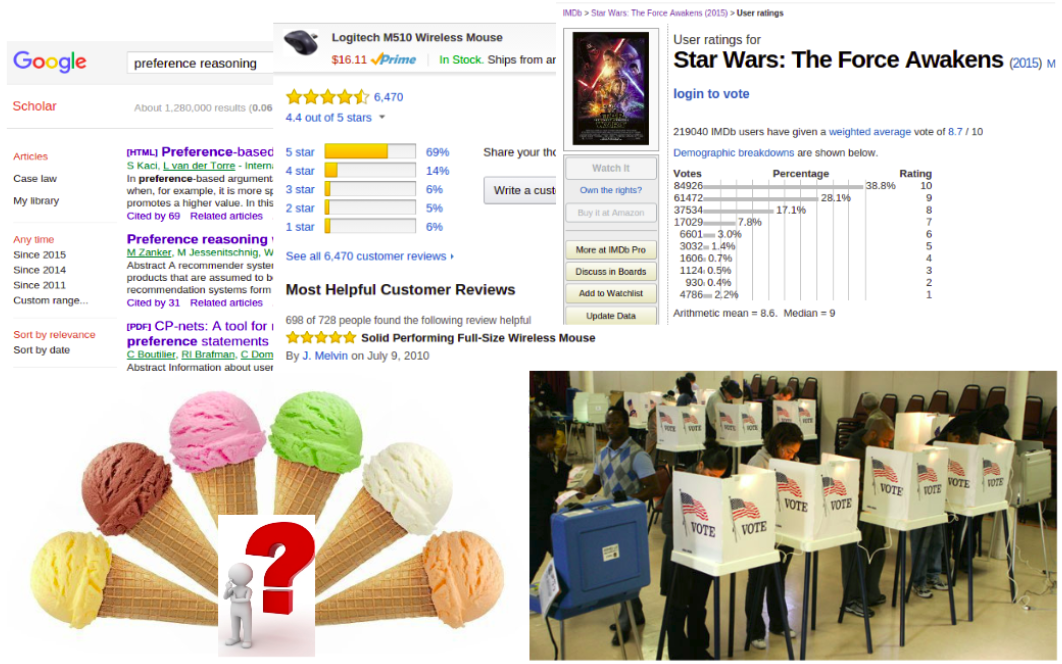
\includegraphics[width=0.8\textwidth]{figs/PrefApplications/pref_applications.png}
	  \caption{Preferences of different forms}
	\end{figure}
}

\frameT{Describing Preferences}{
	\begin{figure}[ht!]
	  \centering
	    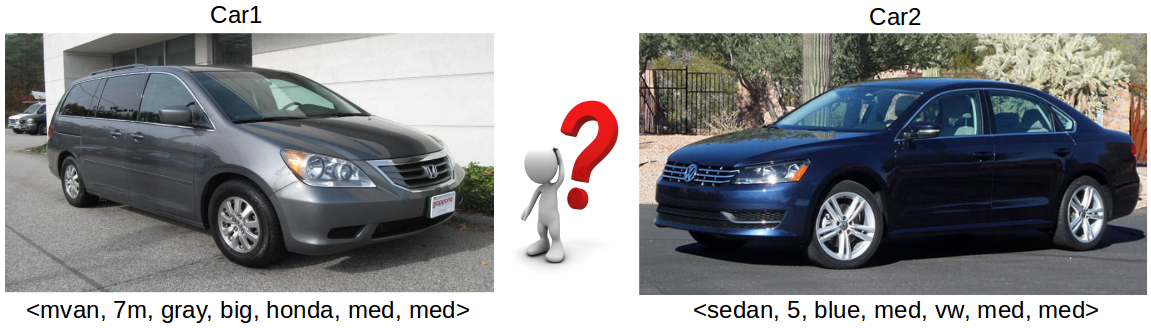
\includegraphics[width=0.95\textwidth]{figs/Cars/individual.png}
	  \caption{How to express preferences?}
	\end{figure}

	\vspace{-0.7cm}

	\begin{enumerate}
		\item How will I rate cars?
		\begin{itemize}
			\item For BodyType, I will assign 7 points to minivans, 5 to sedans, ...
			\item For Color, I will assign 8 points to blue, 4 to gray, ...
		\end{itemize}
		\item What are the desired properties I see in cars?
		\begin{itemize}
			\item I prefer minivans to sedans, ...
			\item If minivan, I prefer gray to blue; if sedan, I prefer blue to gray; ...
		\end{itemize}
	\end{enumerate}
}

\frameT{Describing Preferences}{
	\begin{figure}[ht!]
	  \centering
	    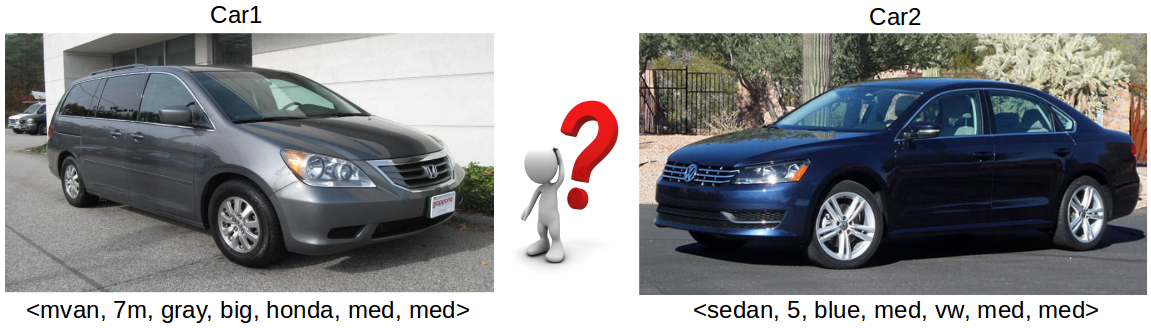
\includegraphics[width=0.95\textwidth]{figs/Cars/individual.png}
	  \caption{How to express preferences?}
	\end{figure}

	\vspace{-0.7cm}

	\begin{enumerate}
		\item How will I rate cars? (\tbf{Quantitative})
		\begin{itemize}
			\item For BodyType, I will assign 7 points to minivans, 5 to sedans, ...
			\item For Color, I will assign 8 points to blue, 4 to gray, ...
		\end{itemize}
		\item What are the desired properties I see in cars? (\tbf{Qualitative})
		\begin{itemize}
			\item I prefer minivans to sedans, ...
			\item If minivan, I prefer gray to blue; if sedan, I prefer blue to gray; ...
		\end{itemize}
	\end{enumerate}
}


\section{Preliminary}
%\frameT{Relations and Orderings}{
%  \begin{block}{Binary Relations}
%		Let $O$ be a set of elements. A \tit{binary relation} $\succeq$ over $O$ is a
%		collection of ordered pairs of elements in $O$; that is,
%		\begin{center}
%			$\succeq \; \subseteq O \times O$.
%		\end{center}
%  \end{block}
%
%	Properties of binary relations related to preferences:
%	\begin{enumerate}
%		\item Reflexivity: $\forall o \in O$, $o\succeq o$.
%		\item Irreflexivity: $\forall o \in O$, $o\not\succeq o$.
%		\item Totality: $\forall o_1,o_2$, $o_1\succeq o_2$ or $o_2\succeq o_1$.
%		\item Transitivity: $\forall o_1,o_2,o_3$, if $o_1\succeq o_2$ and $o_2\succeq o_3$, then $o_1\succeq o_3$.
%		\item Symmetry: $\forall o_1,o_2$, if $o_1\succeq o_2$, then $o_2\succeq o_1$.
%		%\item Asymmetry: $\forall o_1,o_2$, if $o_1\succeq o_2$, then $o_2\not\succeq o_1$.
%		\item Antisymmetry: $\forall o_1,o_2$, if $o_1\succeq o_2$ and $o_2\succeq o_1$, then $o_1=o_2$.
%	\end{enumerate}
%}

\frameT{Relations and Orderings}{
  \begin{block}{Binary Relations}
		Let $O$ be a set of elements. A \tit{binary relation} $R$ over $O$ is a
		collection of ordered pairs of elements in $O$; that is,
		\begin{center}
			$R \subseteq O \times O$.
		\end{center}
  \end{block}

	Properties of binary relations related to preferences:
	{\small
	\begin{enumerate}
		\item Reflexivity: $\forall o \in O$, $(o,o) \in R$.
		\item Irreflexivity: $\forall o \in O$, $(o,o) \not \in R$.
		\item Totality: $\forall o_1,o_2$, $(o_1,o_2) \in R$ or $(o_2,o_1) \in R$.
		\item Transitivity: $\forall o_1,o_2,o_3$, if $(o_1,o_2) \in R$ 
					and $(o_2,o_3) \in R$, then $(o_1,o_3) \in R$.
		\item Symmetry: $\forall o_1,o_2$, if $(o_1,o_2) \in R$, then $(o_2,o_1) \in R$.
		\item Antisymmetry: $\forall o_1,o_2$, if $(o_1,o_2) \in R$ 
					and $(o_2,o_1) \in R$, then $o_1=o_2$.
	\end{enumerate}
	}
}

\frameT{Relations and Orderings}{
  \begin{block}{Orderings}
		%A binary relation $\succeq$ over $O$ 
		$\succeq$
		is a \tit{partial preorder} if it is reflexive and
		transitive, a \tit{total preorder} if it is a partial preorder and total, 
		a \tit{partial order} if it is a partial preorder and antisymmetric, and 
		a \tit{total order} if it is a partial order and total.
  \end{block}

	\vspace{-0.3cm}

	\begin{figure}[ht]
	   \small
	  \centering
    \begin{subfigure}[b]{0.45\textwidth}
	  	\centering
		  \begin{tikzpicture}[->,>=stealth',node distance=1.5cm,main node/.style={circle,draw,font=\small}]
		    \node[main node,inner sep=0pt] (1)                    {$o_1,\!o_5$};
				\node[main node,inner sep=0pt] (2) [below left of=1]  {$o_2,\!o_6$};
		  	\node[main node,inner sep=0pt] (3) [below right of=1] {$o_3,\!o_7$};
		  	\node[main node,inner sep=0pt] (4) [below right of=2] {$o_4,\!o_8$};
		
		    \path[every node/.style={font=\sffamily\small}]
		      (4) edge (2)
		      (4) edge (3)
		      (2) edge (1)
		      (3) edge (1)
		      (4) edge (1)
					(1) edge [loop above] (1)
					(2) edge [loop left] (2)
					(3) edge [loop right] (3)
					(4) edge [loop below] (4);
		  \end{tikzpicture}
      \caption{partial preorder}
    \end{subfigure}
    \begin{subfigure}[b]{0.45\textwidth}
	  	\centering
		  \begin{tikzpicture}[->,>=stealth',node distance=1.1cm,main node/.style={circle,draw,font=\small}]
		    \node[main node,inner sep=0pt] (1)              {$o_1,\!o_5$};
				\node[main node,inner sep=0pt] (2) [below of=1] {$o_2,\!o_6$};
		  	\node[main node,inner sep=0pt] (3) [below of=2] {$o_3,\!o_7$};
		  	\node[main node,inner sep=0pt] (4) [below of=3] {$o_4,\!o_8$};
		
		    \path[every node/.style={font=\sffamily\small}]
		      (4) edge (3)
		      (4) edge [bend left] (2)
		      (4) edge [bend left] (1)
		      (3) edge (2)
		      (3) edge [bend left] (1)
		      (2) edge (1)
					(1) edge [loop right] (1)
					(2) edge [loop right] (2)
					(3) edge [loop right] (3)
					(4) edge [loop right] (4);
		  \end{tikzpicture}
      \caption{total preorder}
    \end{subfigure}
	\end{figure}
}

\frameT{Relations and Orderings}{
  \begin{block}{Orderings}
		%A binary relation $\succeq$ over $O$ 
		$\succeq$
		is a \tit{partial preorder} if it is reflexive and
		transitive, a \tit{total preorder} if it is a partial preorder and total, 
		a \tit{partial order} if it is a partial preorder and antisymmetric, and 
		a \tit{total order} if it is a partial order and total.
  \end{block}

	\vspace{-0.3cm}

	\begin{figure}[ht]
	   \small
	  \centering
    \begin{subfigure}[b]{0.45\textwidth}
	  	\centering
		  \begin{tikzpicture}[->,>=stealth',node distance=1.5cm,main node/.style={circle,draw,font=\small}]
		    \node[main node] (1) {$o_1$};
				\node[main node] (2) [below left of=1] {$o_2$};
		  	\node[main node] (3) [below right of=1] {$o_3$};
		  	\node[main node] (4) [below right of=2] {$o_4$};
		
		    \path[every node/.style={font=\sffamily\small}]
		      (4) edge (2)
		      (4) edge (3)
		      (2) edge (1)
		      (3) edge (1)
		      (4) edge (1)
					(1) edge [loop above] (1)
					(2) edge [loop left] (2)
					(3) edge [loop right] (3)
					(4) edge [loop below] (4);
		  \end{tikzpicture}
      \caption{partial order}
    \end{subfigure}
    \begin{subfigure}[b]{0.45\textwidth}
	  	\centering
		  \begin{tikzpicture}[->,>=stealth',node distance=1cm,main node/.style={circle,draw,font=\small}]
		    \node[main node] (1) {$o_1$};
				\node[main node] (2) [below of=1] {$o_2$};
		  	\node[main node] (3) [below of=2] {$o_3$};
		  	\node[main node] (4) [below of=3] {$o_4$};
		
		    \path[every node/.style={font=\sffamily\small}]
		      (4) edge (3)
		      (4) edge [bend left] (2)
		      (4) edge [bend left] (1)
		      (3) edge (2)
		      (3) edge [bend left] (1)
		      (2) edge (1)
					(1) edge [loop right] (1)
					(2) edge [loop right] (2)
					(3) edge [loop right] (3)
					(4) edge [loop right] (4);
		  \end{tikzpicture}
      \caption{total order}
    \end{subfigure}
	\end{figure}
}

%\frameT{Relations and Orderings}{
%  \begin{block}{Preference Relations}
%		Let $\succeq$ be a preference relation that is a partial preorder over $O$.
%		We say that $o_2$ is \tit{weakly preferred} to $o_1$ if $o_1 \succeq o_2$,
%		that $o_2$ is \tit{strictly preferred} ($\succ$) to $o_1$ if $o_1 \succeq o_2$ and
%		$o_2 \not \succeq o_1$, that $o_1$ is \tit{indifferent} ($\approx$) from $o_2$ 
%		if $o_1 \succeq o_2$ and $o_2 \succeq o_1$, and 
%		that $o_1$ is \tit{incomparable} ($\sim$) with $o_2$ if 
%		$o_1 \not \succeq o_2$ and $o_2 \not \succeq o_1$.
%  \end{block}
%
%	\vspace{-0.3cm}
%
%	\begin{figure}[ht]
%	   \small
%	  \centering
%    \begin{subfigure}[b]{0.45\textwidth}
%	  	\centering
%		  \begin{tikzpicture}[->,>=stealth',node distance=1.5cm,main node/.style={circle,draw,font=\small}]
%		    \node[main node,inner sep=1.2pt] (1)                    {$o_{1,5}$};
%				\node[main node,inner sep=1.2pt] (2) [below left of=1]  {$o_{2,6}$};
%		  	\node[main node,inner sep=1.2pt] (3) [below right of=1] {$o_{3,7}$};
%		  	\node[main node,inner sep=1.2pt] (4) [below right of=2] {$o_{4,8}$};
%		
%		    \path[every node/.style={font=\sffamily\small}]
%		      (4) edge (2)
%		      (4) edge (3)
%		      (2) edge (1)
%		      (3) edge (1)
%		      (4) edge (1)
%					(1) edge [loop above] (1)
%					(2) edge [loop left] (2)
%					(3) edge [loop right] (3)
%					(4) edge [loop below] (4);
%		  \end{tikzpicture}
%			\vspace{-0.3cm}
%      \caption{partial preorder}
%    \end{subfigure}
%    \begin{subfigure}[b]{0.45\textwidth}
%	  	\centering
%			\begin{tikzpicture}[->,>=stealth,node distance=0.5cm,main node/.style={rectangle,font=\small}]
%		    \node[main node] (1)              {$o_1 \succeq o_5$,};
%		    \node[main node] (2) [below of=1] {$o_2 \succ o_4$,};
%		    \node[main node] (3) [below of=2] {$o_4 \approx o_8$,};
%		    \node[main node] (4) [below of=3] {$o_6 \sim o_7$.};
%		    \node[main node] (5) [below of=4] {};
%		    \node[main node] (6) [below of=5] {};
%		  \end{tikzpicture}
%			\vspace{-0.3cm}
%      \caption{preferences}
%    \end{subfigure}
%	\end{figure}
%}

\frameT{Relations and Orderings}{
  \begin{block}{Preference Relations}
		Let $\succeq$ be a preference relation that is a total preorder over $O$.
		We say that $o_1$ is \tit{weakly preferred} to $o_2$ if $o_1 \succeq o_2$,
		that $o_1$ is \tit{strictly preferred} ($\succ$) to $o_2$ if $o_1 \succeq o_2$ and
		$o_2 \not \succeq o_1$, and that $o_1$ is \tit{indifferent} ($\approx$) from $o_2$ 
		if $o_1 \succeq o_2$ and $o_2 \succeq o_1$.
  \end{block}

	\vspace{-0.22cm}

	\begin{figure}[ht]
	   \small
	  \centering
    \begin{subfigure}[b]{0.45\textwidth}
	  	\centering
		  \begin{tikzpicture}[->,>=stealth',node distance=1.1cm,main node/.style={circle,draw,font=\small}]
		    \node[main node,inner sep=0pt] (1)              {$o_1,\!o_5$};
				\node[main node,inner sep=0pt] (2) [below of=1] {$o_2,\!o_6$};
		  	\node[main node,inner sep=0pt] (3) [below of=2] {$o_3,\!o_7$};
		  	\node[main node,inner sep=0pt] (4) [below of=3] {$o_4,\!o_8$};
		
		    \path[every node/.style={font=\sffamily\small}]
		      (4) edge (3)
		      (4) edge [bend left] (2)
		      (4) edge [bend left] (1)
		      (3) edge (2)
		      (3) edge [bend left] (1)
		      (2) edge (1)
					(1) edge [loop right] (1)
					(2) edge [loop right] (2)
					(3) edge [loop right] (3)
					(4) edge [loop right] (4);
		  \end{tikzpicture}
      \caption{total preorder}
    \end{subfigure}
    \begin{subfigure}[b]{0.45\textwidth}
	  	\centering
			\begin{tikzpicture}[->,>=stealth,node distance=0.5cm,main node/.style={rectangle,font=\small}]
		    \node[main node] (1)              {$o_1 \succeq o_5$,};
		    \node[main node] (2) [below of=1] {$o_2 \succ o_4$,};
		    \node[main node] (3) [below of=2] {$o_4 \approx o_8$,};
		    \node[main node] (4) [below of=3] {};
		    \node[main node] (5) [below of=4] {};
		  \end{tikzpicture}
			\vspace{-0.3cm}
      \caption{preferences}
    \end{subfigure}
	\end{figure}
}

\frameT{Combinatorial Domains}
{
	\begin{block}{Combinatorial Domains}
	  Let $V$ be a finite set of variables $\{X_1,\ldots,X_p\}$,
	  associated with a set of finite domains $\{\Dom(X_1),\ldots,\Dom(X_p)\}$ for each
	  variable $X_i$.
	  A \tit{combinatorial domain} $\CD(V)$ is a set of \tit{outcomes}
		described by combinations of values from $\Dom(X_i)$:
	  \begin{center}
	    $\CD(V) = \prod_{X_i \in V} \Dom(X_i)$.
	  \end{center}
	\end{block}
}

\frameT{Combinatorial Domains: Example}{
	Domain of cars over set $V$ of $p$ binary variables:
	\begin{enumerate}
		\item \tbf{BodyType}: \{mvan, sedan\}.
		\item \tbf{Capacity}: \{5, 7m\}.
		\item \tbf{Color}: \{blue, gray\}.
		\item[\vdots]
	\end{enumerate}

	\begin{center}
			$\CD(V) = 
				\underbrace{\{\langle\text{sedan, 5, blue, }\ldots\rangle, 
				\langle\text{mvan, 7m, gray, }\ldots\rangle, \ldots\}}_{\text{\large $2^p$ outcomes, too many!}}$.
	\end{center}

%	\begin{center}
%		\begin{align*} 
%			\CD(V) = \{&<\text{sedan, 4, blue, }\ldots>, \\
%								 &<\text{mvan, 6m, gray, }\ldots>, \\
%								 &\ldots\}.
%		\end{align*}
%	\end{center}
}

%\frameT{Computational Complexity}{
%	\begin{enumerate}
%		\item $P$, $\NP$, $\coNP$: We typically believe that $P \subset \NP$.
%		%\item $\coNP$: problems whose complements are in $\NP$.
%		\item $\deltap{2}$: $P^\NP$, $\sigmap{2}$: $\NP^\NP$, and $\pip{2}$: $\coNP^\NP$.
%		\item $C$-complete: hardest decision problems in class $C$.
%		%\item A decision problem $L$ is $C$-hard if $L' \leq_p L$ for every $L'$ in class $C$.
%		%\item A decision problem $L$ is $C$-complete if $L$ is in class $C$ and $L$ is $C$-hard.
%	\end{enumerate}
%}

%\frameT{Computational Complexity}{
%	\begin{enumerate}
%		\item $P$, $\NP$, $\coNP$: We typically believe that $P \subset \NP$ and $P \subset \coNP$.
%		%\item $\coNP$: problems whose complements are in $\NP$.
%		\item $\deltap{2}$: $P^\NP$, $\sigmap{2}$: $\NP^\NP$, and $\pip{2}$: $\coNP^\NP$.
%		\item $C$-complete: hardest decision problems in class $C$.
%		%\item A decision problem $L$ is $C$-hard if $L' \leq_p L$ for every $L'$ in class $C$.
%		%\item A decision problem $L$ is $C$-complete if $L$ is in class $C$ and $L$ is $C$-hard.
%	\end{enumerate}
%
%	\vspace{-0.3cm}
%
%	\begin{figure}[ht!]
%	  \centering
%	    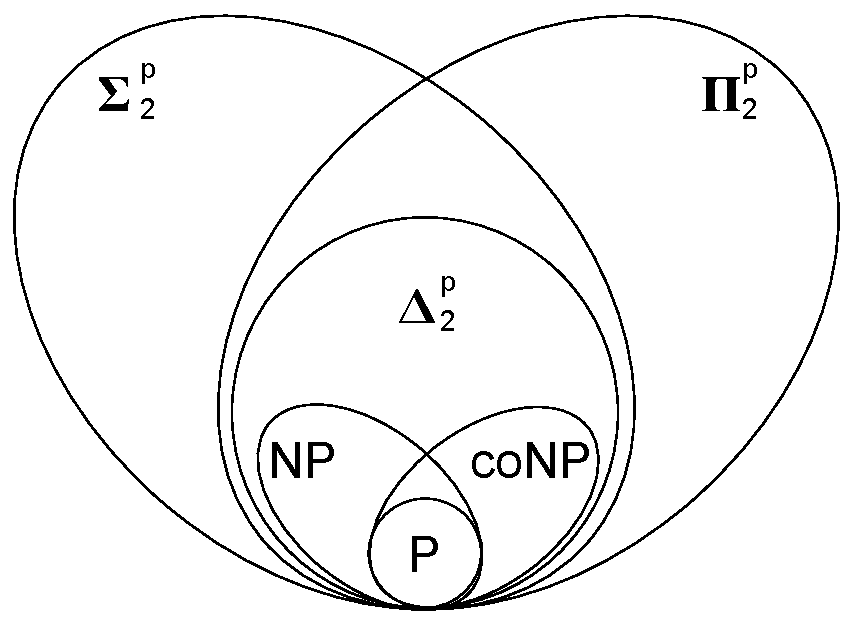
\includegraphics[width=0.5\textwidth]{figs/Preliminary/comp_diagram.pdf}
%	  \caption{Computational complexity diagram}
%	\end{figure}
%}

\frameT{Combinatorial Domains: Example}{
	Domain of cars:
	\begin{enumerate}
		\item \tbf{BodyType}: \{mvan, sedan, sport, suv\}.
		\item \tbf{Capacity}: \{2, 5, 7m\}.
		\item \tbf{Color}: \{black, blue, gray, red, white\}.
		\item \tbf{LuggageSize}: \{big, med, small\}.
		\item \tbf{Make}: \{bmw, ford, honda, vw\}.
		\item \tbf{Price}: \{low, med, high, vhigh\}.
		\item \tbf{Safety}: \{low, med, high\}.
	\end{enumerate}
}

\frameT{Single Agent}{
	\begin{figure}[ht!]
	  \centering
	    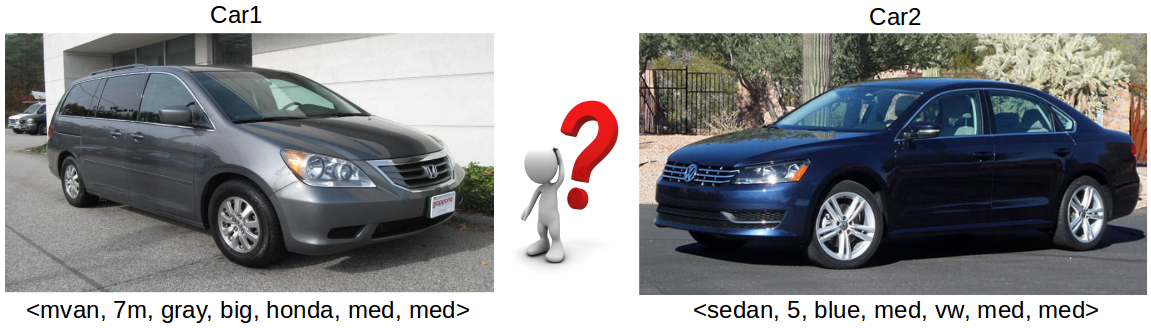
\includegraphics[width=0.95\textwidth]{figs/Cars/individual.png}
	  \caption{Dominance and Optimization}
	\end{figure}
}

\frameT{Multi-Agent}{
	\begin{figure}[ht!]
	  \centering
	    
\includegraphics[width=0.5\textwidth]{figs/Cars/group.png}
	  \caption{Social Choice and Welfare}
	\end{figure}
}

\frameT{Research Problems of Interest}{
	\begin{enumerate}
		\item Preference representation formalisms to compactly model qualitative preferences
					over combinatorial domains.
		\item Preference elicitation and learning methods to cast preferences of agents 
					as a theory in a preference formalism.
		\item Preference reasoning tasks:
		\begin{itemize}
			\item Dominance and optimization
			\item Manipulation: better off by misreporting preferences.
		\end{itemize}
	\end{enumerate}
}


\section{Research Overview}
%\frameT{Research on Preferences}{
%	Q: How do we represent preferences over combinatorial domains?
%
%	\begin{enumerate}
%		\item Quantitative:
%			\begin{enumerate}
%				\item Utility/Cost Functions
%				\item Possibilistic Logic\footcitefull{DuboisLP91}
%				\item Fuzzy Preference Relations\footcitefull{orlovsky1978decision}
%				\item Penalty Logic\footcitefull{pinkas1991propositional}
%			\end{enumerate}
%		\seti
%	\end{enumerate}
%}

%\frameT{Preference Modeling}{
%	Q: How do we compactly represent qualitative preferences over combinatorial domains?
%
%	\begin{enumerate}
%		\item Answer-Set Optimization Theories\footcitefull{Brewka:ASO}
%		\item Ceteris Paribus Networks (e.g., CP-nets\footcitefull{bbdh03},
%					TCP-nets\footcitefull{BrafmanD02:TCP},
%					CI-nets\footcitefull{bouveret2009conditional})
%		\item Conditional Preference Theories\footcitefull{Wilson04extendingcp-nets}
%		\seti
%	\end{enumerate}
%}

\frameT{Preference Modeling}{
	Q: How do we compactly represent qualitative preferences over combinatorial domains?

	\begin{enumerate}
		\item Preference Trees (P-trees)\footcitefull{fraser1994}\textsuperscript{,}\footcitefull{wsh/mpref14/LiuT}
		\item Partial Lexicographic Preference Trees (PLP-trees)\footcitefull{conf/aaai15/LiuT}
		\item Lexicographic Preference Trees (LP-trees)\footcitefull{booth:learningLP}\textsuperscript{,}\footcitefull{conf/adt13/LiuT}
	\end{enumerate}
}

\frameT{Preference Learning}{
	Q: How do we learn predictive qualitative preference models over combinatorial domains?

	\begin{enumerate}
		%\item Ceteris Paribus Networks (e.g., 
		%			CP-nets\footcitefull{lang2009complexity}\textsuperscript{,}\footcitefull{koriche2010learning}\textsuperscript{,}\footcitefull{chevaleyre2011learning})
		%\item Preference Trees (e.g., LP-trees\footcitefull{booth:learningLP}, 
		%			CLP-trees\footcitefull{brauning2012learning}, \tbf{PLP-trees}\footcitefull{conf/aaai15/LiuT})
		\item Partial Lexicographic Preference Trees 
					(PLP-trees)\footcitefull{schmitt2006complexity}\textsuperscript{,}\footcitefull{dombi2007learning}\textsuperscript{,}\footcitefull{conf/aaai15/LiuT}
			\begin{itemize}
				\item Active and passive learning
				\item Compute a (possibly small) PLP-tree consistent with all the data
				\item Compute a PLP-tree that agrees with the data as much as possible
			\end{itemize}
		\item Preference Forests\footcitefull{confInPrep/ijcai16/LiuT1}
		\item Preference Approximation\footcitefull{confInPrep/X/CPN_LPT}
	\end{enumerate}
}

\frameT{Preference Reasoning}{
	Q: How do we reason about preferences over combinatorial domains?

	\begin{enumerate}
		\item Preference Optimization\footcitefull{lang:aggLP}\textsuperscript{,}\footcitefull{conf/adt13/LiuT}\textsuperscript{,}\footcitefull{wsh/mpref14/LiuT}\textsuperscript{,}\footcitefull{conf/adt15/liuT}:
			\begin{itemize}
				\item Dominance testing: $o_1 \succ_P o_2$?
				\item Optimality testing: $o_1 \succ_P o_2$ for all $o_2 \not = o_1$?
				\item Optimality computing: what is the optimal outcome wrt $P$?
				\item Preference aggregation: which candidate wins the election?
			\end{itemize}
		\item Preference Misrepresentation\footcitefull{brandt2012computational}\textsuperscript{,}\footcitefull{confInPrep/X/LiuT}:
			\begin{itemize}
				%\item Control
				\item Manipulation
				%\item Bribery
			\end{itemize}
	\end{enumerate}
}

\frameT{Preference Applications}{
	Q: What fields can we apply preferences to?

	\begin{enumerate}
		\item Game Theory:
			\begin{itemize}
				\item Hedonic games\footcitefull{conf/adt13/Spradling}
			\end{itemize}
		\item Automated Planning and Scheduling:
			\begin{itemize}
				\item Trip planning\footcitefull{abs/parc/Liu1}
			\end{itemize}
		\item Data-Driven Decision Making:
			\begin{itemize}
				\item Predictive decisions\footcitefull{confInPrep/ijcai16/LiuT2}
			\end{itemize}
	\end{enumerate}
}

\frameT{Outline}{
	\begin{enumerate}
		\item The languages of P-trees, PLP-trees, and LP-trees
		\item Learning preference models in case of PLP-trees
		\item Reasoning with preferences:
			\begin{itemize}
				\item Preference optimization in case of P-trees
				\item Computing winners and ``strong" outcomes when votes are LP-trees
				\item Application in trip planning
			\end{itemize}
		\item Future research directions
	\end{enumerate}
}


\section{Preference Modeling}
\frameT{Outline}{
  \begin{enumerate}
    \item The languages of P-trees, PLP-trees, and LP-trees
    {\transparent{0.2} \item Learning of preference models (PLP-trees and P-forests)}
    {\transparent{0.2} \item Reasoning with preferences:
      \begin{itemize}
        \item Computing winners and ``strong" outcomes when votes are LP-trees
        \item Application in trip planning
      \end{itemize}}
    {\transparent{0.2} \item Future research directions}
  \end{enumerate}
}

\frameT{Preference Trees}{
	\begin{enumerate}
		\item Let $\cI=\{X_1,\ldots,X_p\}$ be a set of attributes, and
					$D(\cI)=\{\Dom(X_1),\ldots,\Dom(X_p)\}$ a set of finite domains for $\cI$.
		\item	A \tit{literal} is an assignment to an attribute.  We denote by
					$X_i:=x_{i,j}$ the literal that assigns value $x_{i,j} \in \Dom(X_i)$
					to $X_i$. When no confusion, we write $x_{i,j}$, instead of
					$X_i:=x_{i,j}$, as a literal. 
					We then denote by $\cL=\{x_{i,j} \in \Dom(X_i): X_i \in \cI\}$ the set of
					literals given $\cI$ and $D(\cI)$.
		\item The combinatorial domain $\CD(\cI)$ is defined as earlier.
		\seti
	\end{enumerate}
}

\frameT{Preference Trees}{
	\begin{enumerate}
		\conti
		\item A \tbf{P-tree} $T$ over $\CD(\cI)$
					is a binary tree whose nodes, other than the leaves, are labeled with
					propositional formulas over $\cL$.
		\item Given an outcome $M \in \CD(\cI)$, the \tbf{leaf} $l_T(M)$
					is the leaf reached by traversing the tree $T$ according to $M$.
					When at a node $N$ labeled with $\varphi$, if $M\models \varphi$,
					we descend to the left child of $N$; otherwise, to the right.
		\item For $M, M'\in \CD(\cI)$, we have $M\succ_T M'$ if $l_T(M) \succ_T l_T(M')$,
					and $M \approx_T M'$ if $l_T(M)=l_T(M')$. Outcome $M$ is \tbf{optimal} if 
					there exists no $M'$ such that $M' \succ_T M$.
	\end{enumerate}
}

\frameT{Example: The Cars Domain}{
  \begin{enumerate}
    \item \tbf{BodyType}($X_1$): \{mvan($x_{1,1}$), sedan($x_{1,2}$), sport($x_{1,3}$), suv($x_{1,4}$)\}.
    \item \tbf{Capacity}($X_2$): \{2, 5, 7m\}.
    \item \tbf{Color}($X_3$): \{black, blue, gray, red, white\}.
    \item \tbf{LuggageSize}($X_4$): \{big, med, small\}.
    \item \tbf{Make}($X_5$): \{bmw, ford, honda, and vw\}.
    \item \tbf{Price}($X_6$): \{low, med, high, vhigh\}.
    \item \tbf{Safety}($X_7$): \{low, med, high\}.
  \end{enumerate}
}

\frameT{Example: Preference Trees over Cars}{
	\begin{center}
    \tbf{BodyType}($X_1$): \{mvan($x_{1,1}$), sedan($x_{1,2}$), sport($x_{1,3}$), suv($x_{1,4}$)\}.\\
    \tbf{Color}($X_3$): \{black, blue, gray, red, white\}.\\
    \tbf{Price}($X_6$): \{low, med, high, vhigh\}.
	\end{center}

\vspace{-0.2cm}

	\begin{figure}[!ht]
	  \centering
      \begin{tikzpicture}[->,>=stealth',
	      level 1/.style={sibling distance=1.7cm, level distance=33pt},
	      level 2/.style={sibling distance=1cm, level distance=27pt}
	    ]
        \node [main node,inner sep=4pt] (1){$\varphi$}
          child {node [main node,inner sep=1pt] (2) {$x_{6,2}$}
            child {node [rectangle,draw] (3) {}}
            child {node [rectangle,draw] (4) {}}
                            }
          child {node [main node,inner sep=1pt] (5) {$x_{6,2}$}
            child {node [rectangle,draw] (6) {}
                                    }
            child {node [rectangle,draw] (7) {}
                                    }
          };
      \end{tikzpicture}
	  \caption{A P-tree over cars\footnotemark}
	\end{figure}

	\footnotetext{
		$\varphi=(x_{1,1} \land x_{3,5}) \lor (x_{1,2} \land x_{3,2})$.
	}
}

\frameT{Example: Preferences over Cars}{
	\addtocounter{footnote}{-1}
	\begin{center}
    \tbf{BodyType}($X_1$): \{mvan($x_{1,1}$), sedan($x_{1,2}$), sport($x_{1,3}$), suv($x_{1,4}$)\}.\\
    \tbf{Color}($X_3$): \{black, blue, gray, red, white\}.\\
    \tbf{Price}($X_6$): \{low, med, high, vhigh\}.
	\end{center}

\vspace{-0.2cm}

	\begin{figure}[!ht]
	  \centering
      \begin{tikzpicture}[->,>=stealth',
	      level 1/.style={sibling distance=1.7cm, level distance=33pt},
	      level 2/.style={sibling distance=1cm, level distance=27pt}
	    ]
        \node [main node,inner sep=4pt] (1){$\varphi$}
          child [red] {node [main node,inner sep=1pt,black] (2) {$x_{6,2}$}
            child {node [rectangle,draw,fill] (3) {}}
            child [black] {node [rectangle,draw] (4) {}}
                            }
          child [green] {node [main node,inner sep=1pt,black] (5) {$x_{6,2}$}
            child {node [rectangle,draw,fill] (6) {}
                                    }
            child [black] {node [rectangle,draw] (7) {}
                                    }
          };
      \end{tikzpicture}
	  \caption{A P-tree over cars\footnotemark}
	\end{figure}

\vspace{-1cm}

	\begin{center}
		$\textcolor{red}{Car2} \succ \textcolor{green}{Car1}$
	\end{center}

	\footnotetext{
		$\varphi=(x_{1,1} \land x_{3,5}) \lor (x_{1,2} \land x_{3,2})$.
	}
}

\frameT{Compact Representation of P-trees}{
\begin{figure}[!ht]
	\centering
		\begin{subfigure}[b]{0.75\textwidth}
		\centering
		  \begin{tikzpicture}[->,>=stealth',
  	     level 1/.style={sibling distance=4.3cm, level distance=28pt},
  	     level 2/.style={sibling distance=2.2cm, level distance=28pt},
  	     level 3/.style={sibling distance=1.0cm, level distance=28pt},
  	     level 4/.style={sibling distance=0.5cm, level distance=28pt}]
		    \node [main node,inner sep=1.7pt] (1){$\varphi_1$}
		    child {node [main node,inner sep=1.7pt] (2) {$\varphi_2$}
		      child {node [main node,inner sep=1.7pt] (3) {$\varphi_3$}
		        child {node [main node,inner sep=1.7pt] (4) {$\varphi_4$}
  	          child {node [rectangle,draw] (16) {}}
  	          child {node [rectangle,draw] (17) {}}
						}
		        child {node [main node,inner sep=1.7pt] (5) {$\varphi_4$}
  	          child {node [rectangle,draw] (18) {}}
  	          child {node [rectangle,draw] (19) {}}
						}
					}
		      child {node [main node,inner sep=1.7pt] (6) {$\varphi_3$}
		        child {node [main node,inner sep=1.7pt] (7) {$\varphi_4$}
  	          child {node [rectangle,draw] (20) {}}
  	          child {node [rectangle,draw] (21) {}}
						}
		        child {node [main node,inner sep=1.7pt] (8) {$\varphi_4$}
  	          child {node [rectangle,draw] (22) {}}
  	          child {node [rectangle,draw] (23) {}}
						}
		      }
				}
		    child {node [main node,inner sep=1.7pt] (9) {$\varphi_2$}
		      child {node [main node,inner sep=1.7pt] (10) {$\varphi_3$}
		        child {node [main node,inner sep=1.7pt] (11) {$\varphi_4$}
  	          child {node [rectangle,draw] (24) {}}
  	          child {node [rectangle,draw] (25) {}}
						}
		        child {node [main node,inner sep=1.7pt] (12) {$\varphi_4$}
  	          child {node [rectangle,draw] (26) {}}
  	          child {node [rectangle,draw] (27) {}}
						}
					}
		      child {node [main node,inner sep=1.7pt] (13) {$\varphi_3$}
		        child {node [main node,inner sep=1.7pt] (14) {$\varphi_4$}
  	          child {node [rectangle,draw] (28) {}}
  	          child {node [rectangle,draw] (29) {}}
						}
		        child {node [main node,inner sep=1.7pt] (15) {$\varphi_4$}
  	          child {node [rectangle,draw] (30) {}}
  	          child {node [rectangle,draw] (31) {}}
						}
		      }
				};
		  \end{tikzpicture}
			\caption{Full}
		\end{subfigure}%
		\begin{subfigure}[b]{0.2\textwidth}
			\hspace{0.8cm}
			\begin{tikzpicture}[->,>=stealth',
  	     level 1/.style={sibling distance=4.3cm, level distance=28pt},
  	     level 2/.style={sibling distance=2.2cm, level distance=28pt},
  	     level 3/.style={sibling distance=1.0cm, level distance=28pt},
  	     level 4/.style={sibling distance=0.5cm, level distance=28pt}]
			  \node [main node,inner sep=1.7pt] (1){$\varphi_1$}
			    child {node [main node,inner sep=1.7pt] (3) {$\varphi_2$}
						child {node [main node,inner sep=1.7pt] (4) {$\varphi_3$}
							child {node [main node,inner sep=1.7pt] (5) {$\varphi_4$}
              	child {node [rectangle] (6) {} edge from parent[draw=none]}
							}
						}
					};
			\end{tikzpicture}
			\caption{Compact}
		\end{subfigure}
  \caption{Compact P-trees}
%	\vspace{-0.2cm}
  \label{fig:LPT_full}
\end{figure}
}

\frameT{Compact Representation of P-trees}{
	A \tit{compact P-tree} over $\CD(\cI)$ is a binary tree where
	\begin{enumerate}
		\setlength\itemsep{0em}
		\item every node is labeled with a Boolean formula over $\cI$, and
	  \item every non-leaf node $t$ labeled with $\varphi$ has either
	        two outgoing edges (Figure (a)), or one 
	    		outgoing edge pointing left (Figure (b)),
					right (Figure (c)), or straight-down (Figure (d)).
	\end{enumerate}
	
	\begin{figure}[ht!]
	  \centering
	    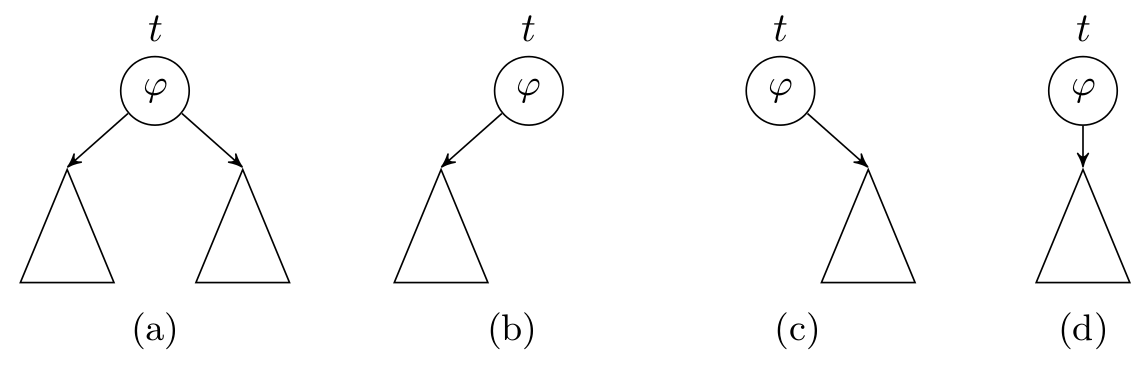
\includegraphics[width=0.9\textwidth]{figs/PTrees/ptrees.png}
	  \caption{Compact P-trees}
	\end{figure}
}

\frameT{Relative Expressivity of Preference Languages}{
	\begin{center}
		Poss-theories = ASO-rules 
		%$\subsetsim$ 
		$\subset$
			\dual{LP-trees/\dual{$\cap$/\dual{PLP-trees/\dual{$\cap$/P-trees}}}}
			$\subset$ ASO-theories
	\end{center}
}

\frameT{Computational Complexity Results}{
	{\sc DomTest}: is it that $o \succeq_T o'$ in P-tree $T$?\\
	{\sc OptTest}: is outcome $o$ optimal w.r.t $T$?\\
	{\sc OptProp}: is there an optimal outcome $o$ w.r.t $T$ st $o \models \alpha$?
	
	\begin{figure}
		\centering

	  \begin{tabular}[0.5\textwidth]{ | c | c | c | c | }
	    \hline
	     & {\sc DomTest}& {\sc OptTest} & {\sc OptProp} \\
			\hline
			LP-tree & P & P & P \\
			\hline
			\pbox{20cm}{ASO-rule/ \\ Poss-theory} & P & coNP-c & $\deltap{2}$($P^{NP}$) \\
	    \hline
	    \tbf{P-tree} & \tbf{P} & \tbf{coNP-c}\fn{The complement problem is reduced from the SAT problem.}
				& \tbf{$\deltap{2}$($P^{NP}$)-c}\fn{The problem is reduced from the Maximum Satisfying 
																					Assignment (MSA) problem.}\\
			\hline
			ASO-theory & P & coNP-c & $\sigmap{2}$($NP^{NP}$)-c \\
	    \hline
			%ACP-net & NP-hard & P & P \\
	    %\hline
			%CCP-net & PSPACE-c & PSPACE-c? & PSPACE-c? \\
	    %\hline
	  \end{tabular}

		\caption{Computational complexity results}

	\end{figure}
}

\frameT{Partial Lexicographic Preference Trees (PLP-Tree)}{
	A \tit{PLP-tree} over $\CD(\cI)$ is a tree, where
	\begin{enumerate}
		\setlength\itemsep{0em}
		\item every node $t$ is labeled with an attribute $\Attr(t)$ in $\cI$ and
					a conditional preference table $\CPT(t)$,
	  \item every non-leaf node $t$ has either one unlabeled outgoing edge or multiple
					outgoing edges labeled, each labeled by some value in $\Dom(\Attr(t))$, and
		\item every attribute appears \tit{at most} once on every branch.
	\end{enumerate}
}

\frameT{Partial Lexicographic Preference Trees (PLP-Tree)}{
	\begin{figure}[ht!]
	  \centering
	    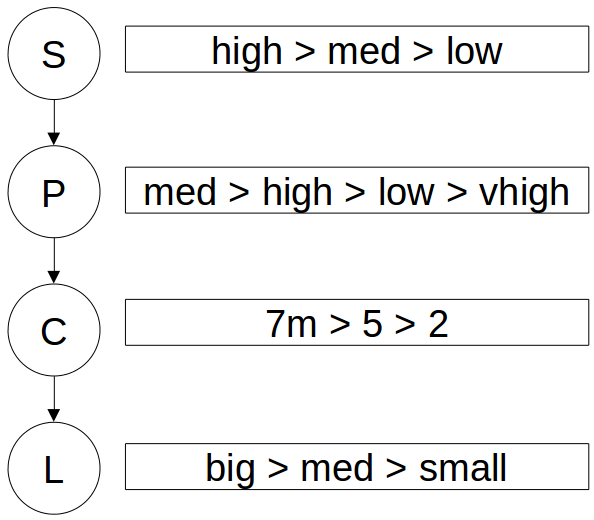
\includegraphics[width=0.4\textwidth]{figs/Cars/uiuptree.png}
	  \caption{A UIUP PLP-tree}
	\end{figure}

	According to this UIUP PLP-tree, \tit{Car1} is preferred to \tit{Car2}.
}

\frameT{Partial Lexicographic Preference Trees (PLP-Tree)}{
	\begin{figure}[ht!]
	  \centering
	    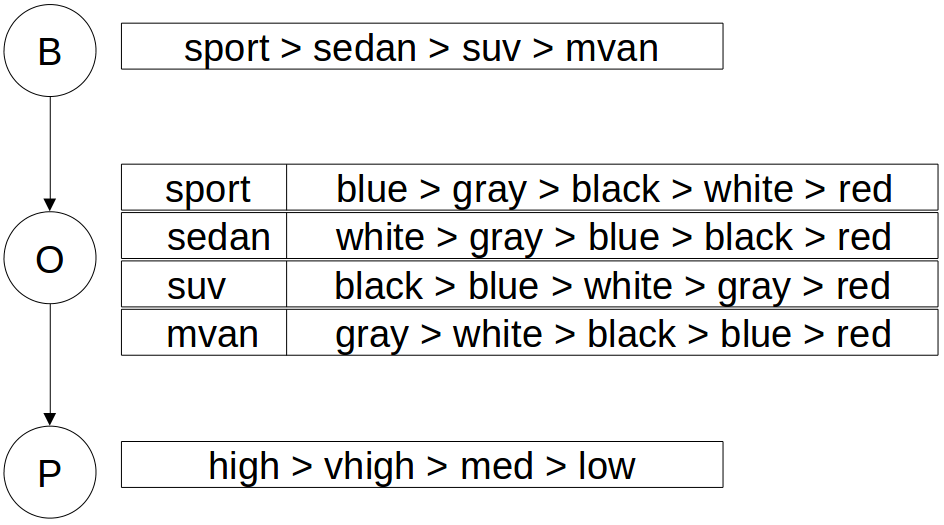
\includegraphics[width=0.65\textwidth]{figs/Cars/uicptree.png}
	  \caption{A UICP PLP-tree}
	\end{figure}

	According to this UICP PLP-tree, \tit{Car2} is preferred to \tit{Car1}.
}

\frameT{Partial Lexicographic Preference Trees (PLP-Tree)}{
	\begin{figure}[ht!]
	  \centering
	    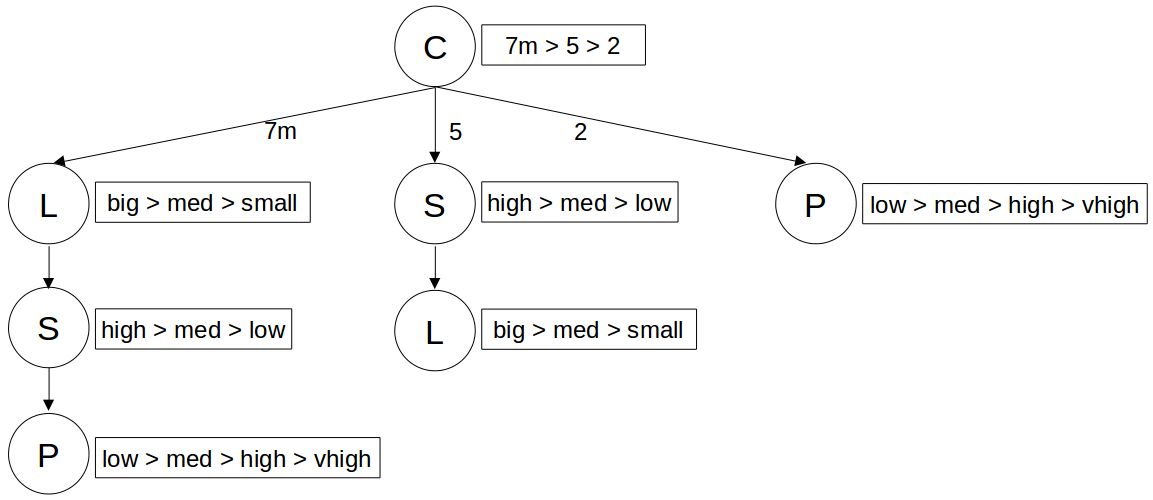
\includegraphics[width=0.9\textwidth]{figs/Cars/ciuptree.png}
	  \caption{A CIUP PLP-tree}
	\end{figure}

	According to this CICP PLP-tree, \tit{Car1} is preferred to \tit{Car2}.
}

\frameT{Partial Lexicographic Preference Trees (PLP-Tree)}{
	\begin{figure}[ht!]
	  \centering
	    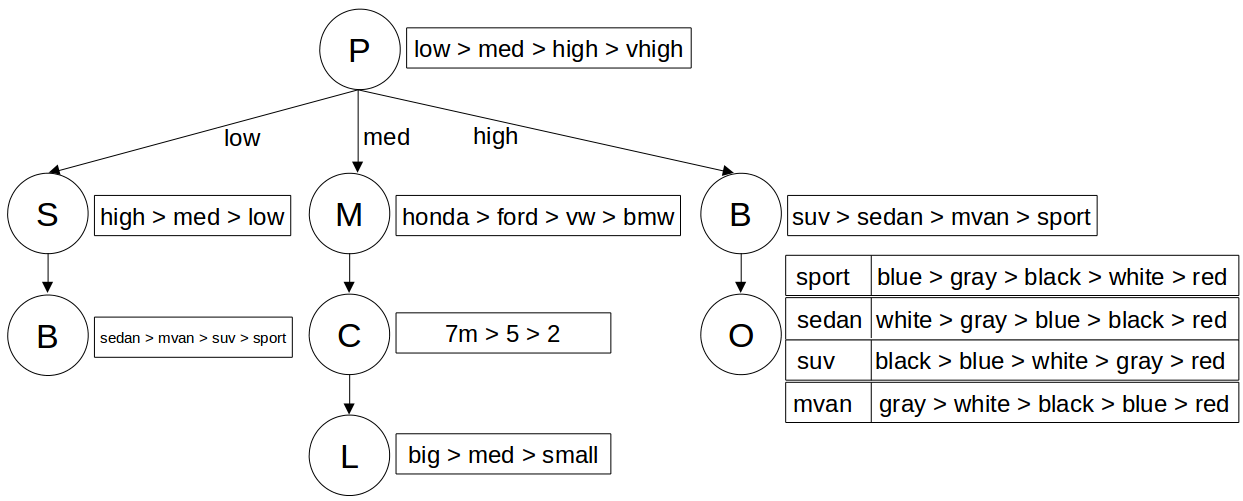
\includegraphics[width=0.9\textwidth]{figs/Cars/cicptree.png}
	  \caption{A CICP PLP-tree}
	\end{figure}

	According to this CICP PLP-tree, \tit{Car1} is preferred to \tit{Car2}.
}

\frameT{Lexicographic Preference Trees (LP-Trees)}
{
  \begin{enumerate}
    \item An \tit{LP-tree} $\cL$ over $\CD(\cI)$ is a PLP-tree, where
    \begin{itemize}
      \item each attribute appears \tbf{exactly once} on every path from the root to a leaf.
    \end{itemize}
  \end{enumerate}
}


\section{Preference Learning}
\frameT{Outline}{
  \begin{enumerate}
    {\transparent{0.2} \item The languages of PLP-trees and LP-trees}
    \item Learning preference models in case of PLP-trees
    {\transparent{0.2} \item Reasoning with preferences:
      \begin{itemize}
        \item Computing winners and ``strong" candidates when votes are LP-trees
        \item Application in trip planning
      \end{itemize}}
    {\transparent{0.2} \item Future research directions}
  \end{enumerate}
}

\frameT{The Cars Domain}{
  \begin{enumerate}
    \item \tbf{BodyType}(B): \{mvan, sedan, sport, suv\}.
    \item \tbf{Capacity}(C): \{2, 5, 7m\}.
    \item \tbf{Color}(O): \{black, blue, gray, red, white\}.
    \item \tbf{LuggageSize}(L): \{big, med, small\}.
    \item \tbf{Make}(M): \{bmw, ford, honda, vw\}.
    \item \tbf{Price}(P): \{low, med, high, vhigh\}.
    \item \tbf{Safety}(S): \{low, med, high\}.
  \end{enumerate}
}

\frameT{Learning PLP-trees}{
	\begin{block}{Consistent Learning (\tsc{ConsLearn})}
		Given an example set $\cE$, decide 
		whether there exists a PLP-tree $T$ (of a particular type) such that $T$ 
		is consistent with $\cE$.
	\end{block}
	\vspace{-0.3cm}

  \begin{figure}[ht]
     \small
    \centering
    \begin{subfigure}[b]{0.95\textwidth}
      \centering
      \begin{tikzpicture}[->,>=stealth,node distance=0.5cm,main node/.style={rectangle,font=\small}]
        \node[main node] (1)              {\textcolor{blue}{($<$sdn,5,blk,m,h,m,m$>$,$<$suv,7m,wht,b,f,m,m$>$)}}; 
        \node[main node] (2) [below of=1] {\textcolor{green}{($<$spt,2,wht,s,bmw,h,h$>$,$<$spt,2,wht,s,bmw,vh,h$>$)}};
        \node[main node] (3) [below of=2] {\textcolor{magenta}{($<$mvn,7m,gry,b,f,m,m$>$,$<$sdn,5,bl,m,f,m,m$>$)}};
      \end{tikzpicture}
      %\caption{Examples}
    \end{subfigure}\\ \vspace{0.5cm}
    \begin{subfigure}[b]{0.95\textwidth}
    	\centering
      \begin{tikzpicture}[->,>=stealth',
        level 1/.style={sibling distance=2cm, level distance=33pt},
        level 2/.style={sibling distance=0.7cm, level distance=27pt}
      ]

        \node[main node,inner sep=2pt] (1) {P};
        \node[rectangle,draw,inner sep=2pt] at (1.2,0) {\textcolor{green}{$m \!\!>\!\! h\!\!>\!\! l\!\!>\!\! vh$}};

        \node[main node,inner sep=2pt] (2) [below of=1] {M};
        \node[rectangle,draw,inner sep=2pt] at (1.52,-1) {\textcolor{blue}{$h \!\!>\!\! vw\!\!>\!\! f\!\!>\!\! bmw$}};

        \node[main node,inner sep=2pt] (3) [below of=2] {B};
        \node[rectangle,draw,inner sep=2pt] at (1.8,-2) {\textcolor{magenta}{$mvn\!\! >\!\! suv\!\! >\!\! sdn\!\! >\!\! spt$}};

        \path[every node/.style={font=\sffamily\small}]
          (1) edge (2)
          (2) edge (3);
      \end{tikzpicture}
      \caption*{UIUP tree}
    \end{subfigure}
  \end{figure}
}

\frameT{Learning PLP-trees}{
	\begin{block}{Small Learning (\tsc{SmallLearn})}
		Given an example set $\cE$
		and a positive integer $l$ ($l \leq |\cE|$), decide whether there 
		exists a PLP-tree $T$ (of a particular type) such that $T$ is consistent 
		with $\cE$ and $|T| \leq l$.
	\end{block}
	\vspace{-0.3cm}

  \begin{figure}[ht]
     \small
    \centering
    \begin{subfigure}[b]{0.95\textwidth}
      \centering
      \begin{tikzpicture}[->,>=stealth,node distance=0.5cm,main node/.style={rectangle,font=\small}]
        \node[main node] (1)              {\textcolor{blue}{($<$sdn,5,blk,m,h,m,m$>$,$<$suv,7m,wht,b,f,m,m$>$)}}; 
        \node[main node] (2) [below of=1] {\textcolor{green}{($<$spt,2,wht,s,bmw,h,h$>$,$<$spt,2,wht,s,bmw,vh,h$>$)}};
        \node[main node] (3) [below of=2] {\textcolor{blue}{($<$mvn,7m,gry,b,f,m,m$>$,$<$sdn,5,bl,m,f,m,m$>$)}};
      \end{tikzpicture}
      %\caption{Examples}
    \end{subfigure}\\ \vspace{0.5cm}
    \begin{subfigure}[b]{0.95\textwidth}
    	\centering
      \begin{tikzpicture}[->,>=stealth',
        level 1/.style={sibling distance=2cm, level distance=33pt},
        level 2/.style={sibling distance=0.7cm, level distance=27pt}
      ]

        \node[main node,inner sep=2pt] (1) {B};
        \node[rectangle,draw,inner sep=2pt] at (1.8,0) {\textcolor{blue}{$mvn\!\! >\!\! sdn\!\! >\!\! suv\!\! >\!\! spt$}};

        \node[main node,inner sep=2pt] (2) [below of=1] {P};
        \node[rectangle,draw,inner sep=2pt] at (1.2,-1) {\textcolor{green}{$m \!\!>\!\! h\!\!>\!\! l\!\!>\!\! vh$}};

        \path[every node/.style={font=\sffamily\small}]
          (1) edge (2);
      \end{tikzpicture}
      \caption*{UIUP tree}
    \end{subfigure}
  \end{figure}
}

\frameT{Learning PLP-trees}{
	\begin{block}{Maixmal Learning (\tsc{MaxLearn})}
		Given an example set $\cE$ and a 
		positive integer $k$ ($k \leq m$), decide whether there exists a PLP-tree 
		$T$ (of a particular type) such that $T$ satisfies at least $k$ examples 
		in $\cE$.
	\end{block}
	\vspace{-0.3cm}

  \begin{figure}[ht]
     \small
    \centering
    \begin{subfigure}[b]{0.95\textwidth}
      \centering
      \begin{tikzpicture}[->,>=stealth,node distance=0.5cm,main node/.style={rectangle,font=\small}]
        \node[main node] (1)              {\textcolor{blue}{($<$sdn,5,blk,m,h,m,m$>$,$<$suv,7m,wht,b,f,m,m$>$)}}; 
        \node[main node] (2) [below of=1] {\textcolor{green}{($<$spt,2,wht,s,bmw,h,h$>$,$<$spt,2,wht,s,bmw,vh,h$>$)}};
        \node[main node] (3) [below of=2] {\textcolor{blue}{($<$mvn,7m,gry,b,f,m,m$>$,$<$sdn,5,bl,m,f,m,m$>$)}};
        \node[main node] (4) [below of=3] {\textcolor{red}{($<$suv,7m,gry,b,vw,vh,m$>$,$<$suv,7m,gry,b,vw,h,m$>$)}};
      \end{tikzpicture}
      %\caption{Examples}
    \end{subfigure}\\ \vspace{0.5cm}
    \begin{subfigure}[b]{0.95\textwidth}
    	\centering
      \begin{tikzpicture}[->,>=stealth',
        level 1/.style={sibling distance=2cm, level distance=33pt},
        level 2/.style={sibling distance=0.7cm, level distance=27pt}
      ]

        \node[main node,inner sep=2pt] (1) {B};
        \node[rectangle,draw,inner sep=2pt] at (1.8,0) {\textcolor{blue}{$mvn\!\! >\!\! sdn\!\! >\!\! suv\!\! >\!\! spt$}};

        \node[main node,inner sep=2pt] (2) [below of=1] {P};
        \node[rectangle,draw,inner sep=2pt] at (1.2,-1) {\textcolor{green}{$m \!\!>\!\! h\!\!>\!\! l\!\!>\!\! vh$}};

        \path[every node/.style={font=\sffamily\small}]
          (1) edge (2);
      \end{tikzpicture}
      \caption*{UIUP tree}
    \end{subfigure}
  \end{figure}
}

\frameT{Learning PLP-trees}{
	\begin{block}{Consistent Learning (\tsc{ConsLearn})}
		Given an example set $\cE$, decide 
		whether there exists a PLP-tree $T$ (of a particular type) such that $T$ 
		is consistent with $\cE$.
	\end{block}
	\vspace{-0.3cm}

  \begin{figure}[ht]
     \small
    \centering
    \begin{subfigure}[b]{0.95\textwidth}
      \centering
      \begin{tikzpicture}[->,>=stealth,node distance=0.5cm,main node/.style={rectangle,font=\small}]
        \node[main node] (1)              {\textcolor{blue}{($<$sdn,5,blk,m,h,m,m$>$,$<$suv,7m,wht,b,f,m,m$>$)}}; 
        \node[main node] (2) [below of=1] {\textcolor{green}{($<$spt,2,wht,s,bmw,h,h$>$,$<$spt,2,wht,s,bmw,vh,h$>$)}};
        \node[main node] (3) [below of=2] {\textcolor{blue}{($<$mvn,7m,gry,b,f,m,m$>$,$<$sdn,5,bl,m,f,m,m$>$)}};
        \node[main node] (4) [below of=3] {\textcolor{red}{($<$suv,7m,gry,b,vw,vh,m$>$,$<$suv,7m,gry,b,vw,h,m$>$)}};
      \end{tikzpicture}
      %\caption{Examples}
    \end{subfigure}\\ \vspace{0.5cm}
    \begin{subfigure}[b]{0.95\textwidth}
    	\centering
      \begin{tikzpicture}[->,>=stealth',
        level 1/.style={sibling distance=2cm, level distance=33pt},
        level 2/.style={sibling distance=0.7cm, level distance=27pt}
      ]

        \node[main node,inner sep=2pt] (1) {B};
        \node[rectangle,draw,inner sep=2pt] at (1.8,0) {\textcolor{blue}{$mvn\!\! >\!\! sdn\!\! >\!\! suv\!\! >\!\! spt$}};

        \node[main node,inner sep=2pt] (2) [below of=1] {P};
        \node[rectangle split, rectangle split parts=4, draw,inner sep=2pt,font=\sffamily\small] at (1.6,-1.5)
            {
              \textcolor{green}{$spt\!:m \!\!>\!\! h\!\!>\!\! l\!\!>\!\! vh$}
              \nodepart{second}
              \textcolor{red}{$suv\!:vh \!\!>\!\! h\!\!>\!\! m\!\!>\!\! l$}
              \nodepart{third}
              $mvn\!:\!m \!\!>\!\! h\!\!>\!\! l\!\!>\!\! vh$
              \nodepart{fourth}
              $sdn\!:\!m \!\!>\!\! h\!\!>\!\! l\!\!>\!\! vh$
            };

        \path[every node/.style={font=\sffamily\small}]
          (1) edge (2);
      \end{tikzpicture}
      \caption*{UICP tree}
    \end{subfigure}
  \end{figure}
}

%\frameT{Learning PLP-trees}{
%	\begin{block}{Consistent Learning (\tsc{ConsLearn})}
%		Given an example set $\cE$, decide 
%		whether there exists a PLP-tree $T$ (of a particular type) such that $T$ 
%		is consistent with $\cE$.
%	\end{block}
%
%	\begin{block}{Small Learning (\tsc{SmallLearn})}
%		Given an example set $\cE$
%		and a positive integer $l$ ($l \leq |\cE|$), decide whether there 
%		exists a PLP-tree $T$ (of a particular type) such that $T$ is consistent 
%		with $\cE$ and $|T| \leq l$.
%	\end{block}
%
%	\begin{block}{Maixmal Learning (\tsc{MaxLearn})}
%		Given an example set $\cE$ and a 
%		positive integer $k$ ($k \leq m$), decide whether there exists a PLP-tree 
%		$T$ (of a particular type) such that $T$ satisfies at least $k$ examples 
%		in $\cE$.
%	\end{block}
%}

\frameT{Computational Complexity}{
  \begin{enumerate}
    \item $P$, $\NP$, $\coNP$: We typically believe that $P \subset \NP$ and $P \subset \coNP$.
    %\item $\coNP$: problems whose complements are in $\NP$.
    \item $\deltap{2}$: $P^\NP$, $\sigmap{2}$: $\NP^\NP$, and $\pip{2}$: $\coNP^\NP$.
    \item $C$-complete: hardest decision problems in class $C$.
    %\item A decision problem $L$ is $C$-hard if $L' \leq_p L$ for every $L'$ in class $C$.
    %\item A decision problem $L$ is $C$-complete if $L$ is in class $C$ and $L$ is $C$-hard.
  \end{enumerate}

  \vspace{-0.3cm}

  \begin{figure}[ht!]
    \centering
      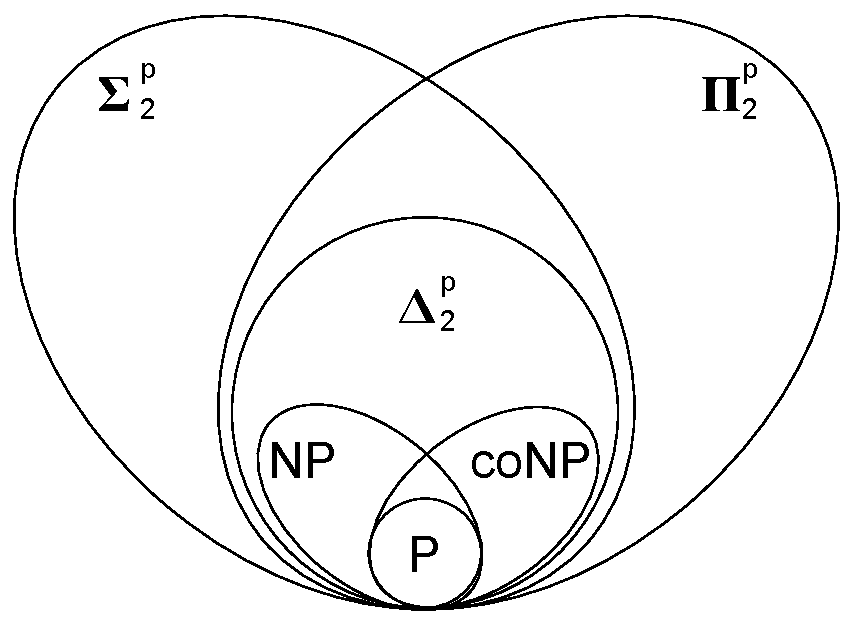
\includegraphics[width=0.5\textwidth]{figs/Preliminary/comp_diagram.pdf}
    \caption{Computational complexity diagram}
  \end{figure}
}

\frameT{Complexity Results on PLP-trees} {
  \begin{figure}[!ht]
    \centering
    \begin{subfigure}[b]{0.45\textwidth}
      \centering
      \begin{tabular}[0.45\textwidth]{ | c | c | c | }
        \hline
           & UP & CP \\
        \hline
        UI & P & P\\
        \hline
        CI & NPC\footnotemark & P  \\
        \hline
      \end{tabular}
      \caption{\tsc{ConsLearn}}
    \end{subfigure}
      \footnotetext{\scriptsize Booth et al., \tit{Learning Conditionally Lexicographic
            Preference Relations}, 2010.}
    \begin{subfigure}[b]{0.45\textwidth}
      \centering
      \begin{tabular}[0.45\textwidth]{ | c | c | c | }
        \hline
           & UP & CP \\
        \hline
        UI & NPC & NPC \\
        \hline
        CI & NPC & NPC \\
        \hline
      \end{tabular}
      \caption{\tsc{SmallLearn}}
    \end{subfigure} \\
    \begin{subfigure}[b]{0.45\textwidth}
      \centering
      \begin{tabular}[0.45\textwidth]{ | c | c | c | }
        \hline
           & UP & CP \\
        \hline
        UI & NPC\footnotemark & NPC \\
        \hline
        CI & NPC & NPC \\
        \hline
      \end{tabular}
      \caption{\tsc{MaxLearn}}
    \end{subfigure}
    \caption{Complexity results for learning PLP-trees}
  \end{figure}
  \footnotetext{\scriptsize Schmitt and Martignon, \tit{On the Complexity of
            Learning Lexicographic Strategies}, 2006.}
}

\frameT{Experimentation}{
  \begin{figure}[ht!]
    \centering
      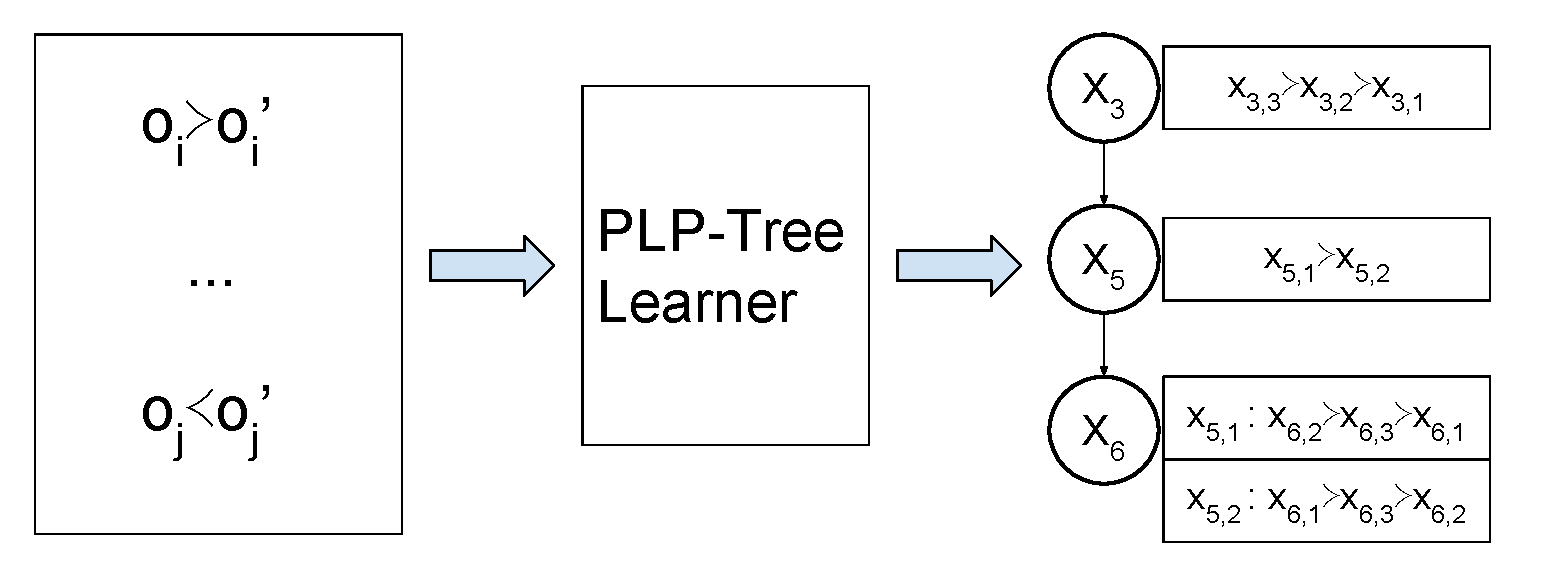
\includegraphics[width=0.9\textwidth]{figs/PrefLearnResults/LearningPLPT.pdf}
    \caption{PLP-tree learning system}
  \end{figure}

}

\frameT{Datasets}{
	\begin{figure}
		\centering
		\begin{tabular}{ |c||c|c|c|c| } 
			\hline
			Dataset          & \#Attributes & \#Objects & \#Examples \\
			\hline \hline
			BreastCancerWisconsin   & 9 & 270 & 9,009 \\ 
			\hline
			CarEvaluation           & 6 & 1,728 & 682,721 \\ 
			\hline
			CreditApproval          & 10 & 520 & 66,079 \\
			\hline
			GermanCredit            & 10 & 914 & 172,368  \\
			\hline
			Ionosphere              & 10 & 118 & 3,472 \\
			\hline
			MammographicMass        & 5 & 62 & 792 \\
			\hline
			Mushroom                & 10 & 184 & 8,448 \\
			\hline
			Nursery                 & 8 & 1,266 & 548,064 \\
			\hline
			SPECTHeart              & 10 & 115 & 3,196 \\
			\hline
			TicTacToe               & 9 & 958 & 207,832 \\
			\hline
			Vehicle                 & 10 & 455 & 76,713 \\
			\hline
			Wine                    & 10 & 177 & 10,322 \\
			\hline
		\end{tabular}
		\caption{Preference Learning Library\footnotemark}
	\end{figure}

	\footnotetext{\tiny \url{http://www.cs.uky.edu/~liu/preflearnlib.php}}
}

\frameT{PLP-Trees To Learn}{
  \begin{figure}[ht!]
    \centering
      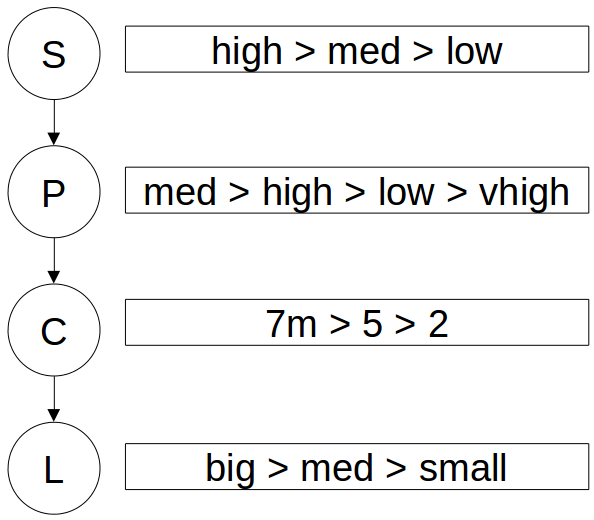
\includegraphics[width=0.4\textwidth]{figs/Cars/uiuptree.png}
    \caption{Unconditional Importance \& Unconditional Preference (UIUP)}
  \end{figure}
}

\frameT{PLP-Trees To Learn}{
  \begin{figure}[ht!]
    \centering
      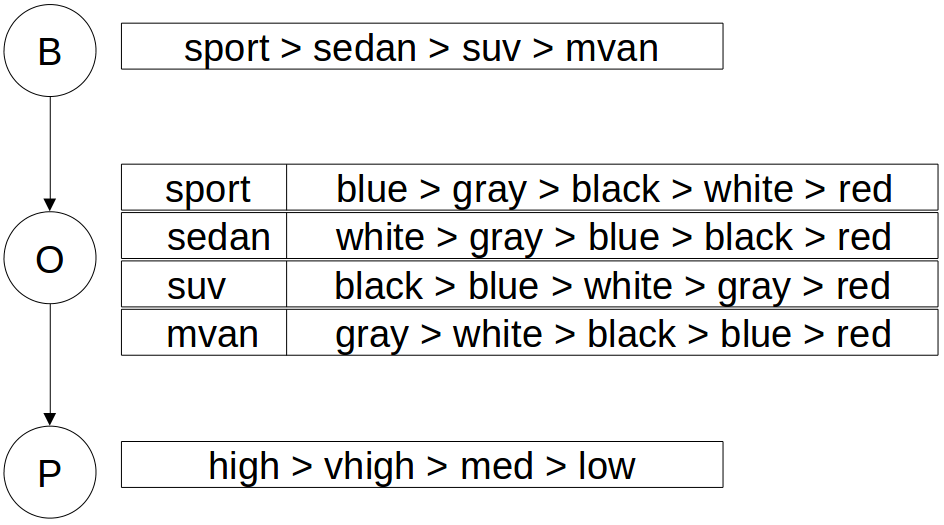
\includegraphics[width=0.65\textwidth]{figs/Cars/uicptree.png}
    \caption{UICP with at most 1 parent (UICP-1)}
  \end{figure}
}

\frameT{PLP-Trees To Learn}{
  \begin{figure}[ht!]
    \centering
      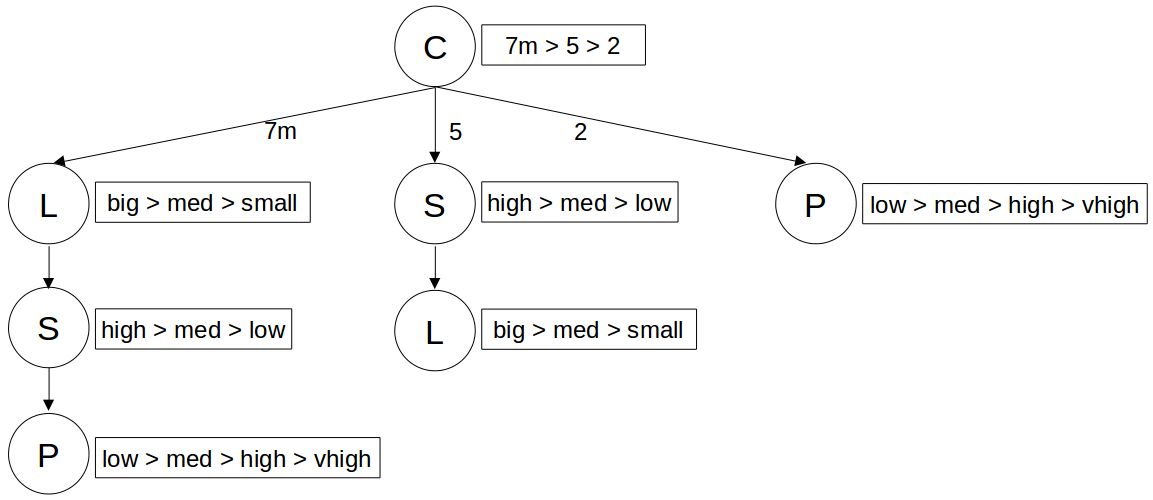
\includegraphics[width=0.9\textwidth]{figs/Cars/ciuptree.png}
    \caption{CIUP with 1 split at the root (CIUP-1)}
  \end{figure}
}

\frameT{PLP-Trees To Learn}{
  \begin{figure}[ht!]
    \centering
      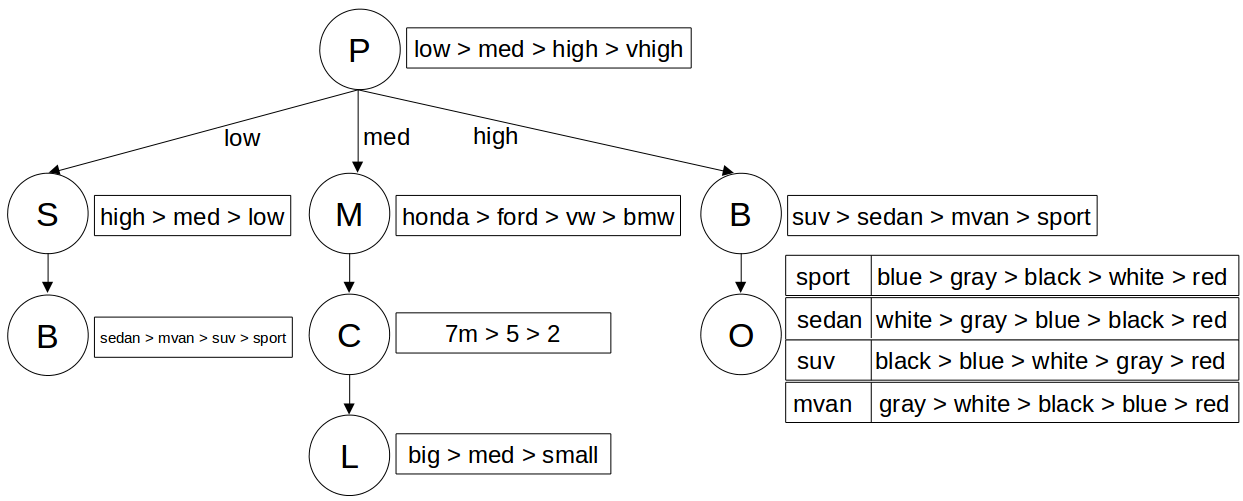
\includegraphics[width=0.9\textwidth]{figs/Cars/cicptree.png}
    \caption{Simple CICP (SCICP)}
  \end{figure}
}

\frameT{Experimental Results: CarEvaluation\footnote{
\tiny \url{http://www.cs.uky.edu/~liu/preflearnlib.php}}
}
{
	\begin{center}
		\#attributes:6, \#objects:1728, \#examples:682721
	\end{center}

  \begin{figure}
    \centering
    \begin{subfigure}[b]{0.48\textwidth}
      \centering
      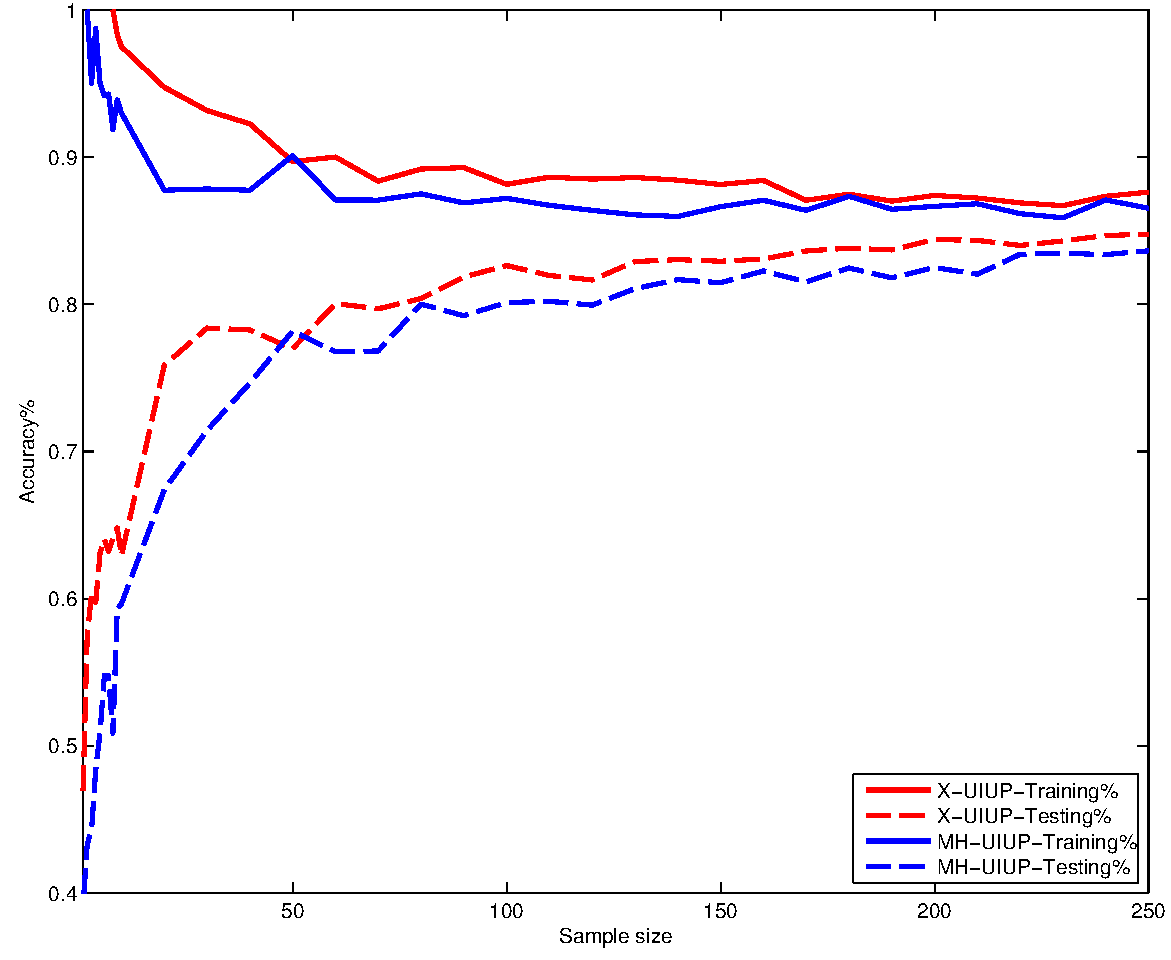
\includegraphics[width=0.95\textwidth]{figs/PrefLearnResults/MatLabOutput/CarEvaluation_Trees_X_MH.pdf}
      \caption{Compare exact \& greedy heuristic}
    \end{subfigure}
    \begin{subfigure}[b]{0.48\textwidth}
      \centering
      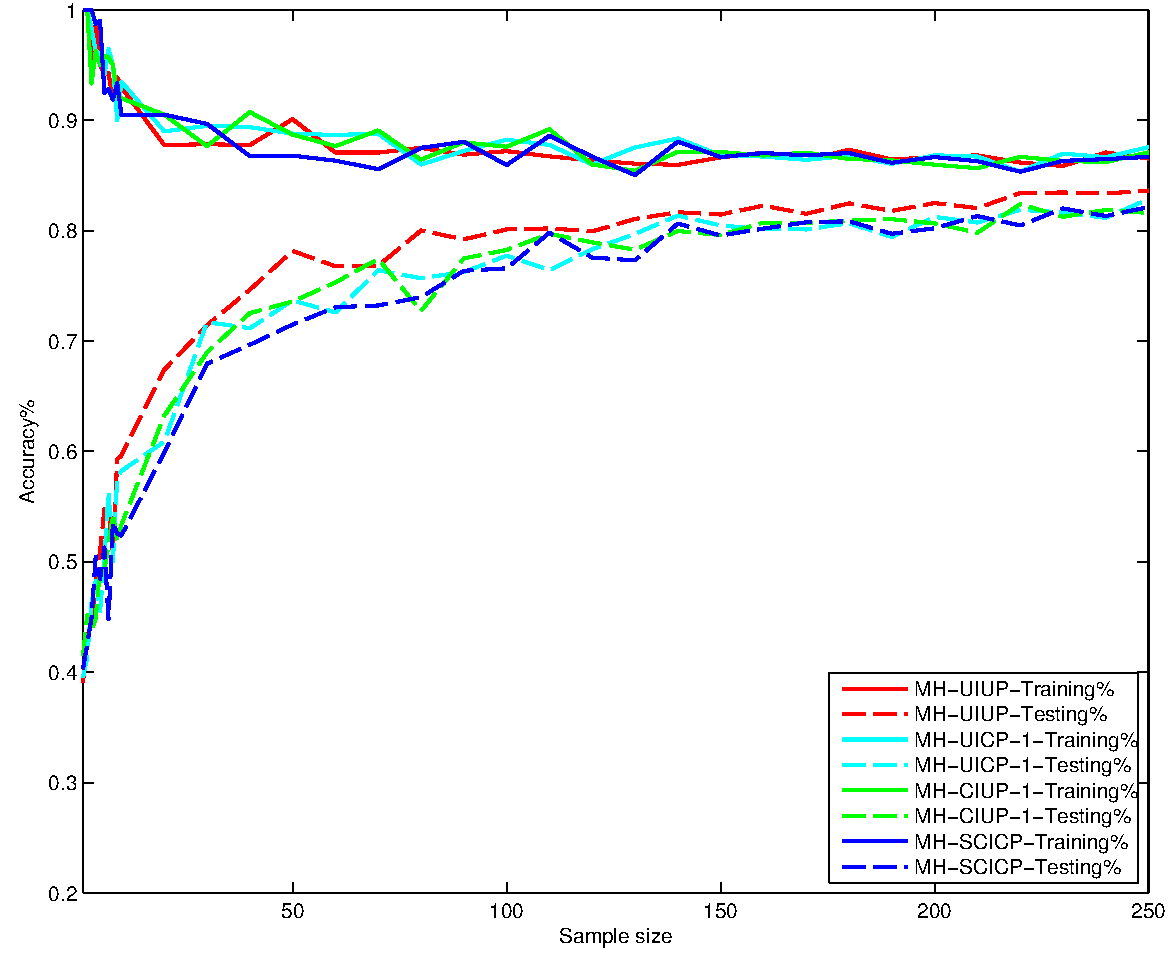
\includegraphics[width=0.95\textwidth]{figs/PrefLearnResults/MatLabOutput/CarEvaluation_Trees_MH.pdf}
      \caption{Greedy heuristic}
    \end{subfigure}

    \caption{Learning curves solving \tsc{MaxLearn}}
  \end{figure}
}

\frameT{Experimental Results: Wine\footnote{
\tiny \url{http://www.cs.uky.edu/~liu/preflearnlib.php}}
}
{
	\begin{center}
		\#attributes:10, \#objects:177, \#examples:10322
	\end{center}

  \begin{figure}
    \centering
    \begin{subfigure}[b]{0.48\textwidth}
      \centering
      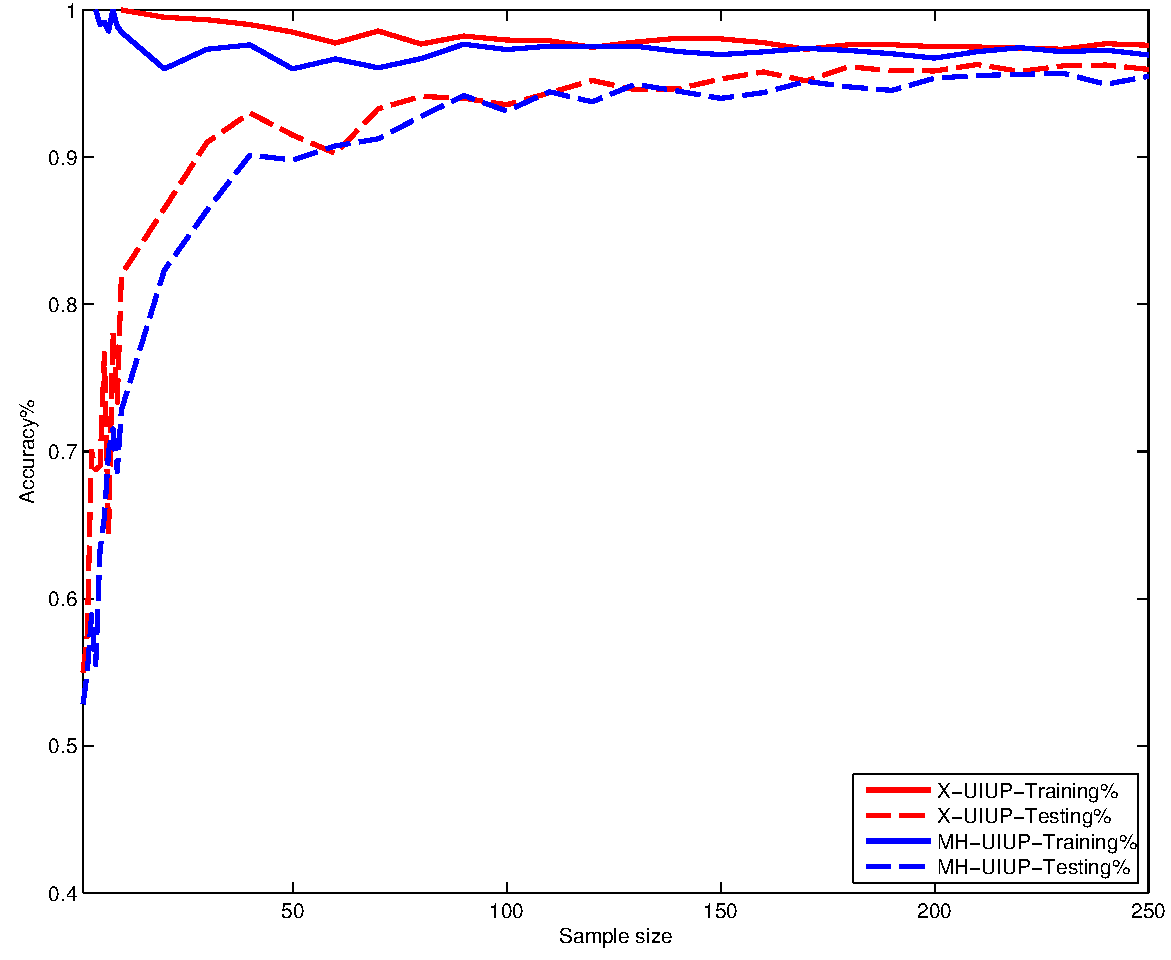
\includegraphics[width=0.95\textwidth]{figs/PrefLearnResults/MatLabOutput/Wine_Trees_X_MH.pdf}
      \caption{Compare exact \& greedy heuristic}
    \end{subfigure}
    \begin{subfigure}[b]{0.48\textwidth}
      \centering
      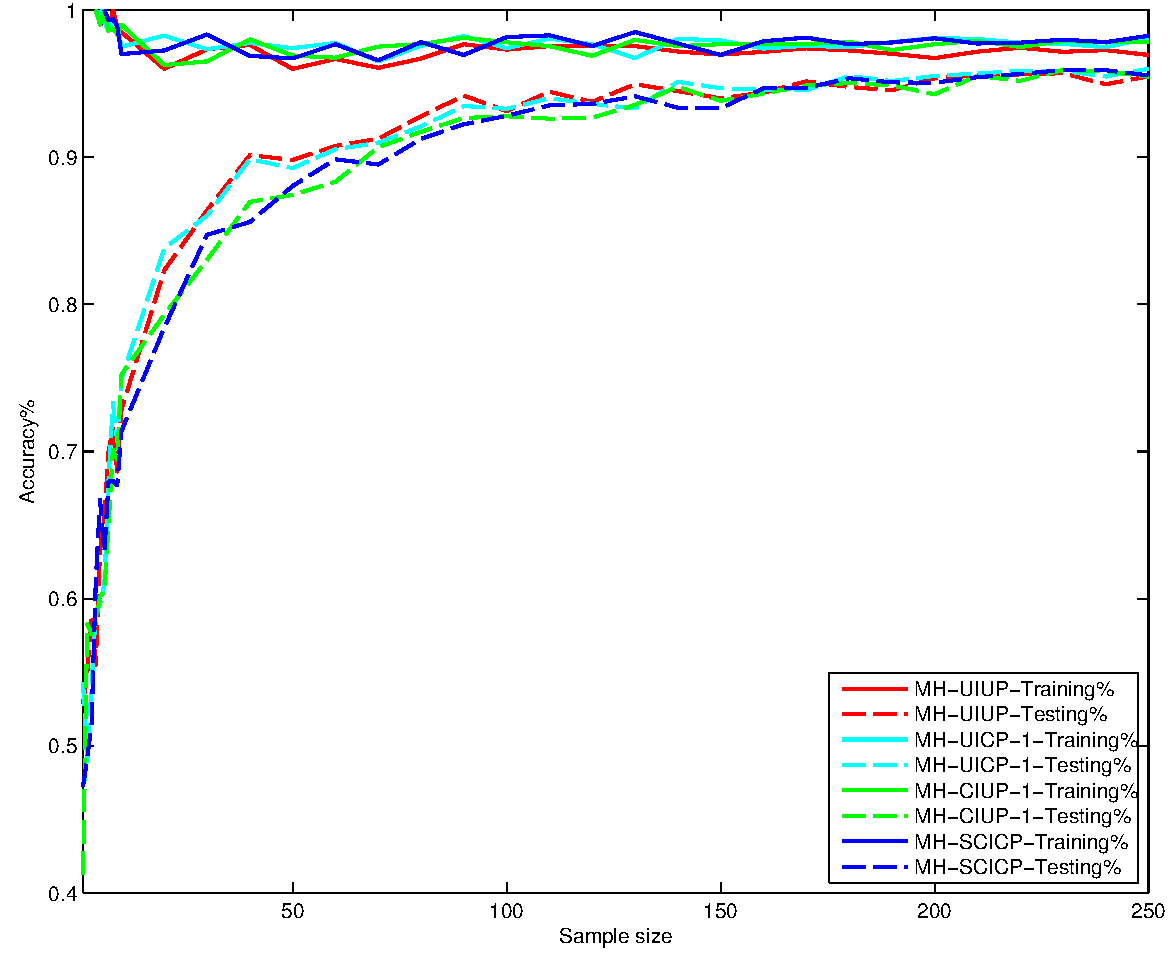
\includegraphics[width=0.95\textwidth]{figs/PrefLearnResults/MatLabOutput/Wine_Trees_MH.pdf}
      \caption{Greedy heuristic}
    \end{subfigure}

    \caption{Learning curves solving \tsc{MaxLearn}}
  \end{figure}
}

%\frameT{Preference Forests (P-Forests)}{
%	\begin{enumerate}
%		\item A \tit{preference forest} $F$ is a collection of PLP-trees
%					$F = \{T_1,\ldots,T_n\}$.
%		\item Denote by $N_F(o_1,o_2)=|\{T \in F:o_1 \succ_T o_2\}|$.
%		\item Given a preference forest $F$, and two outcomes $o_1$ and $o_2$, 
%					we say that $o_1 \succ_F^\Maj o_2$ iff $N_F(o_1,o_2)>N_F(o_2,o_1)$,
%					and that $o_1 \approx_F^\Maj o_2$ iff $N_F(o_1,o_2)=N_F(o_2,o_1)$.
%		\begin{itemize}
%			\item Pro: intuitive, decided in polynomial time.
%			\item Con: Condorcet paradox.
%			\item Other aggregating rules: positional scoring rules, Copeland's method, etc.
%		\end{itemize}
%	\end{enumerate}
%}
%
%\frameT{Experimental Results on P-Forests}{
%  \begin{figure}[ht!]
%    \centering
%      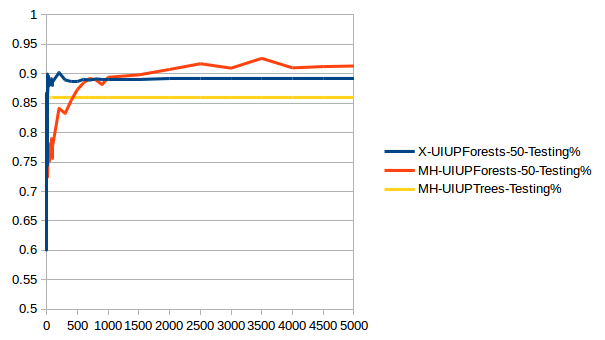
\includegraphics[width=0.7\textwidth]{figs/PrefLearnResults/Forests/X_MH/CarEvaluation.png}
%    \caption{Learning UIUP using ASP and greedy heuristic}
%  \end{figure}
%}
%
%\frameT{Experimental Results on P-Forests}{
%  \begin{figure}[ht!]
%    \centering
%      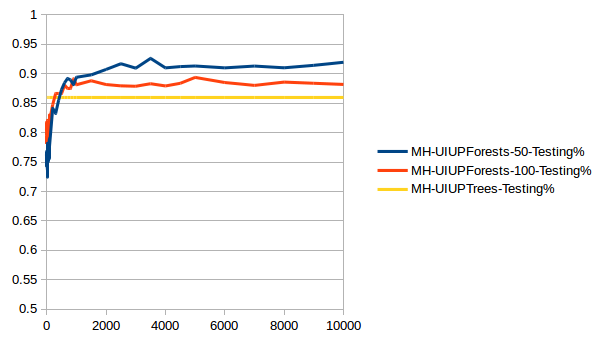
\includegraphics[width=0.7\textwidth]{figs/PrefLearnResults/Forests/MH/CarEvaluation.png}
%    \caption{Learning all four classes using greedy heuristic}
%  \end{figure}
%}


\section{Preference Reasoning on LP-trees}
%\frameT{Outline}{
%  \begin{enumerate}
%    {\transparent{0.2} \item The languages of P-trees, PLP-trees, and LP-trees}
%    {\transparent{0.2} \item Learning preference models in case of PLP-trees}
%    \item Reasoning with preferences:
%      \begin{itemize}
%        \item Preference optimization in case of P-trees
%        {\transparent{0.2} \item Computing winners and ``strong" candidates when votes are LP-trees}
%        {\transparent{0.2} \item Application in trip planning}
%      \end{itemize}
%    {\transparent{0.2} \item Future research directions}
%  \end{enumerate}
%}
%
%\frameT{Computational Complexity Results for P-trees}{
% Dominance-testing ({\sc DomTest}): $o_1 \succ_T o_2$?\\
% Optimality-testing ({\sc OptTest}): $o$ optimal w.r.t $T$?\\
% Optimality-with-property ({\sc OptProp}): is there optimal $o$ 
% with property $\alpha$?
%
% \begin{enumerate}
%   \item {\sc DomTest}$\;\in P$
%   \item {\sc OptTest}$\;\in \coNP$-complete:
%     \begin{itemize}
%       \item The complement problem is reduced from the SAT problem.
%     \end{itemize}
%   \item {\sc OptProp}$\;\in \deltap{2}$-complete:
%     \begin{itemize}
%       \item The problem is reduced from the Maximum Satisfying Assignment (MSA) problem. 
%     \end{itemize}
% \end{enumerate}
%}

\frameT{Outline}{
  \begin{enumerate}
    {\transparent{0.2} \item The languages of PLP-trees and LP-trees}
    {\transparent{0.2} \item Learning preference models in case of PLP-trees}
    \item Reasoning with preferences:
      \begin{itemize}
        \item Computing winners and ``strong" candidates when votes are LP-trees
        {\transparent{0.2} \item Application in trip planning}
      \end{itemize}
    {\transparent{0.2} \item Future research directions}
  \end{enumerate}
}

\frameT{Positional Scoring Rules}
{
	\begin{itemize}
		\item $k$-approval: ($1,\ldots,1,0,\ldots,0$) with $k$ being the number
					of $1$'s.
		\item $(k,l)$-approval: $(c,\ldots, c, d,\ldots, d, 0\ldots, 0)$,
		      where $c$ and $d$ are constants ($c>d$),
					and the numbers of $c$'s and $d$'s equal to $k$ and $l$.
		\item $b$-Borda: ($b, b-1, \ldots, b-m+1$), where $b$ is a constant and
					$m$ is the number of candidates.
	\end{itemize}
}

\frameT{The Evaluation and Winner Problems}
{
  \begin{block}{The Evaluation Problem}
		Let $r$ be a positional scoring rule with a scoring 
		vector $w$, $\cC$ a class of LP-trees.
		Given a $\cC$-profile $P$ of $n$ LP-trees over $p$ attributes and a 
		positive integer $R$,
		the \tit{evaluation} problem is to decide whether 
		there exists an alternative $o \in \mathcal{X}$ such that $s_{{w}}(o,P)
    \geq R$.
  \end{block}

	\vspace{0.5cm}

  \begin{block}{The Winner Problem}
		Let $r$ be a positional scoring rule with a scoring 
		vector $w$, $\cC$ a class of LP-trees.
		Given a $\cC$-profile $P$ of $n$ LP-trees over $p$ attributes,
		the \tit{winner} problem is to compute an alternative
		$o \in \cX$ with the maximum score $s_w(o,P)$.
  \end{block}
}

\frameT{Complexity of the Evaluation Problem: $k$-Approval}
{
	\begin{figure}
		\centering
    \begin{subfigure}[b]{0.45\textwidth}
			\centering
		  \begin{tabular}[0.45\textwidth]{ | c | c | c | }
		    \hline
		      & UP & CP \\
		    \hline
		    UI & P & P \\
		    \hline
		    CI & P & P \\
		    \hline
		  \end{tabular}
			\caption{\footnotesize $k=2^{p-1} \pm f(p)$, $f(p)$ is a poly}
		\end{subfigure}
    \begin{subfigure}[b]{0.45\textwidth}
			\centering
		  \begin{tabular}[0.45\textwidth]{ | c | c | c | }
		    \hline
		      & UP & CP \\
		    \hline
		    UI & NPC & NPC \\
		    \hline
		    CI & NPC & NPC \\
		    \hline
		  \end{tabular}
			\caption{\footnotesize $k=2^{p-c}$, $c>1$ is a const}
		\end{subfigure}
		\caption{$k$-Approval}
	\end{figure}
%	mutiple of high order of 2
}

\frameT{Complexity of the Evaluation Problem: $(k,l)$-Approval}
{
	\begin{figure}
		\centering
    \begin{subfigure}[b]{0.45\textwidth}
			\centering
		  \begin{tabular}[0.45\textwidth]{ | c | c | c | }
		    \hline
		      & UP & CP \\
		    \hline
		    UI & P & P \\
		    \hline
		    CI & P & P \\
		    \hline
		  \end{tabular}
			\caption{$k=l=2^{p-1}$}
		\end{subfigure}
    \begin{subfigure}[b]{0.45\textwidth}
			\centering
		  \begin{tabular}[0.45\textwidth]{ | c | c | c | }
		    \hline
		      & UP & CP \\
		    \hline
		    UI & NPC & NPC \\
		    \hline
		    CI & NPC & NPC \\
		    \hline
		  \end{tabular}
			\caption{\footnotesize $k=l=2^{p-c}$, $c>1$ is a const}
		\end{subfigure}
		\caption{$(k,l)$-Approval}
	\end{figure}
}

\frameT{Complexity of the Evaluation Problem: $b$-Borda}
{
	\begin{figure}
		\centering
    \begin{subfigure}[b]{0.45\textwidth}
			\centering
		  \begin{tabular}[0.45\textwidth]{ | c | c | c | }
		    \hline
		      & UP & CP \\
		    \hline
		    UI & P & NPC \\
		    \hline
		    CI & NPC & NPC \\
		    \hline
		  \end{tabular}
			\caption{$b = 2^p-1$}
		\end{subfigure}
    \begin{subfigure}[b]{0.45\textwidth}
			\centering
		  \begin{tabular}[0.45\textwidth]{ | c | c | c | }
		    \hline
		      & UP & CP \\
		    \hline
		    UI & NPC & NPC \\
		    \hline
		    CI & NPC & NPC \\
		    \hline
		  \end{tabular}
			\caption{\footnotesize $b = 2^{p-c}-1$, $c\geq 1$ is a const}
		\end{subfigure}
		\caption{$b$-Borda}
	\end{figure}
}

\frameT{Modeling the Problems in ASP}
{
	\begin{figure}
		\centering
		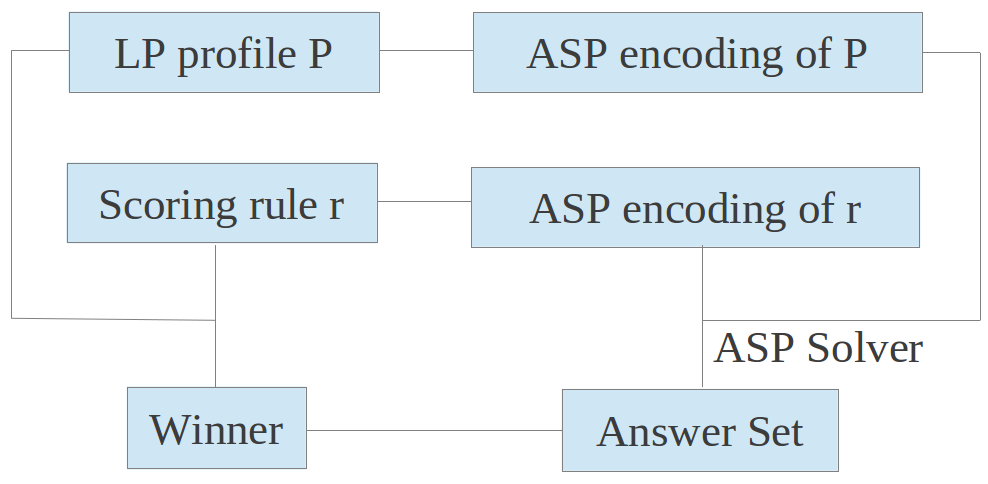
\includegraphics[width=8cm,height=3.8cm]{figs/LPTrees/asp_win_struct.png}
		\caption{The winner problem}
	\end{figure}

	\vspace{-0.45cm}

	\begin{itemize}
		\item Solvers: \tit{clingo}\footcitefull{Gebser:clingo}, 
					\tit{clingcon}\footcitefull{Ostrowski:clingcon}
	\end{itemize}
}

\frameT{Modeling the Problems in W-MAXSAT}
{
	\begin{figure}
		\centering
		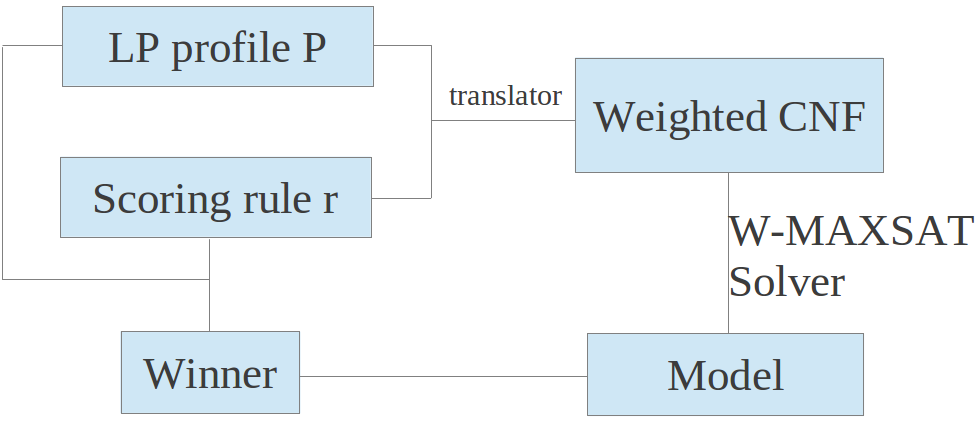
\includegraphics[width=8cm,height=3.6cm]{figs/LPTrees/sat_win_struct.png}
		\caption{The winner problem}
	\end{figure}

	\vspace{-0.45cm}

	\begin{itemize}
		\item Solver: \tit{toulbar}\footcitefull{sanchez2008max}
	\end{itemize}
}

%\frameT{Random LP Profiles}
%{
%	\begin{itemize}
%		\item To experiment with LP profiles, we developed methods to randomly generate
%					\tit{encodings} of
%          a special type of CI-CP LP-tree of size linear in the number of
%          attributes
%	\end{itemize}
%
%	\begin{figure}
%		\vspace{-0.2cm}
%		\centering
%		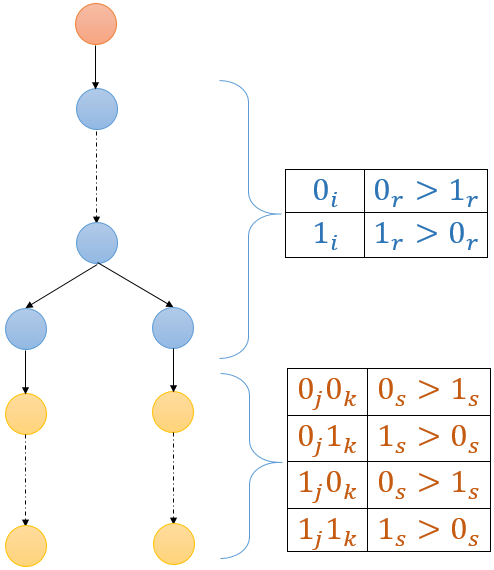
\includegraphics[width=0.4\textwidth]{figs/LPTrees/simple_LP_tree.png}
%		\vspace{-0.3cm}
%		\caption{Random LP-tree}
%	\end{figure}
%}

\frameT{Varying $p$ and $n$: $2^{p-2}$-approval}
{
	\begin{figure}
		\centering
    \begin{subfigure}[b]{0.45\textwidth}
			\centering
			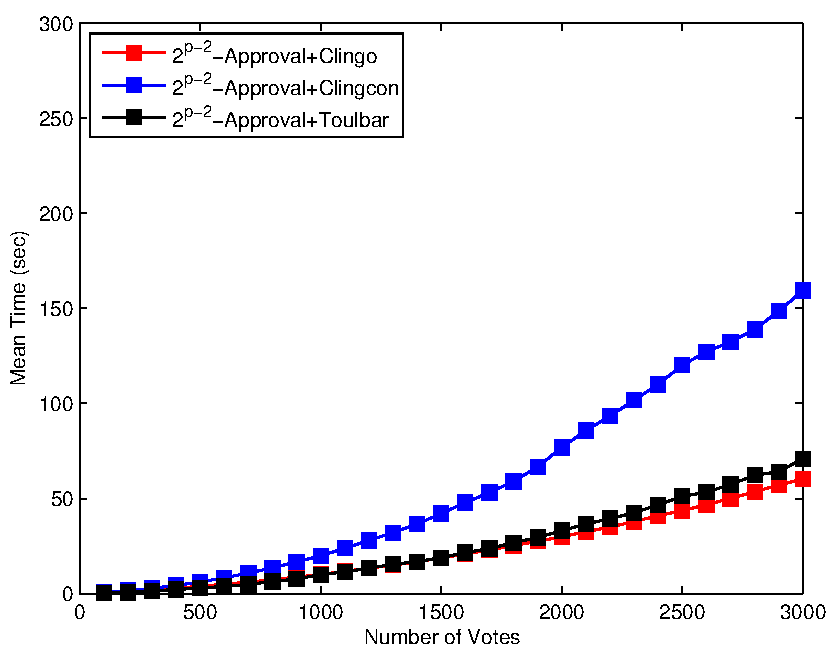
\includegraphics[width=0.95\textwidth]{figs/LPTrees/win/expAppFISCICP.pdf}
			\caption{Fixed \#attributes (10)}
		\end{subfigure}
    \begin{subfigure}[b]{0.45\textwidth}
			\centering
			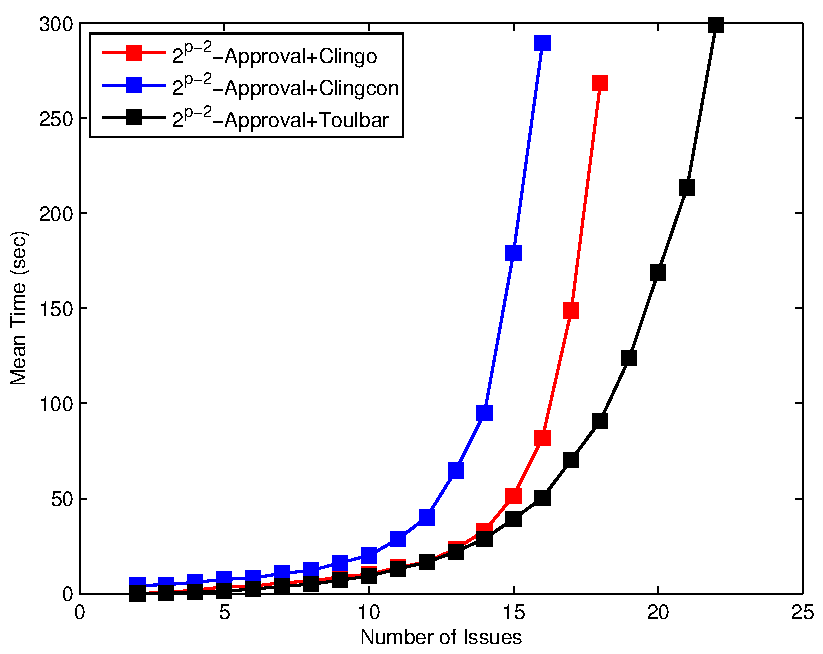
\includegraphics[width=0.95\textwidth]{figs/LPTrees/win/expAppFVSCICP.pdf}
			\caption{Fixed \#votes (1000)}
		\end{subfigure}

		\caption{Solving the winner problem}
	\end{figure}
}

\frameT{Varying $p$ and $n$: ($2^{p-2},2^{p-2}$)-approval
	\fn{
		scoring vector: ($2,\ldots,2,1,\ldots,1,0,\ldots,0$) with the numbers
		of 2's and 1's equal to $2^{p-2}$
	}}
{
	\begin{figure}
		\centering
    \begin{subfigure}[b]{0.45\textwidth}
			\centering
			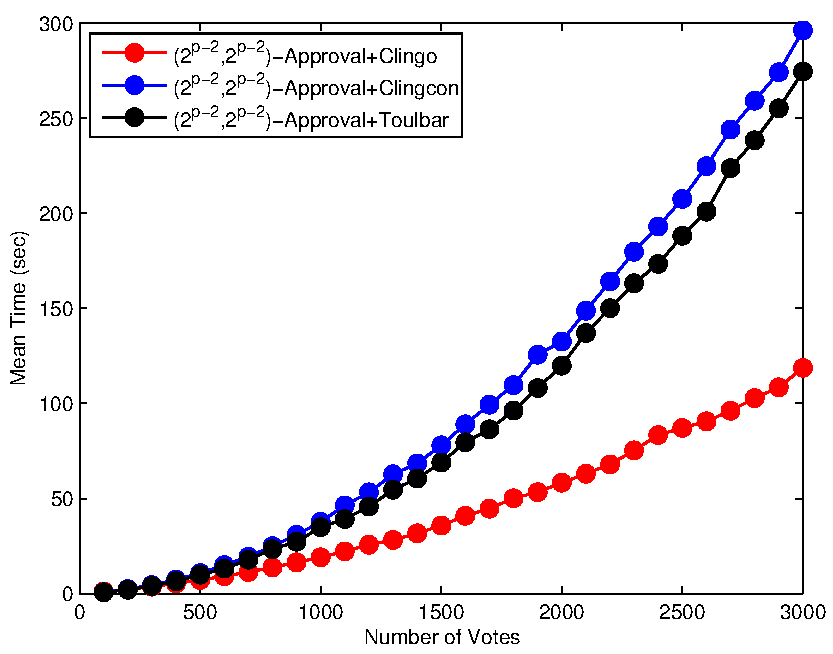
\includegraphics[width=0.95\textwidth]{figs/LPTrees/win/2kAppFISCICP.pdf}
			\caption{Fixed \#attributes (10)}
		\end{subfigure}
    \begin{subfigure}[b]{0.45\textwidth}
			\centering
			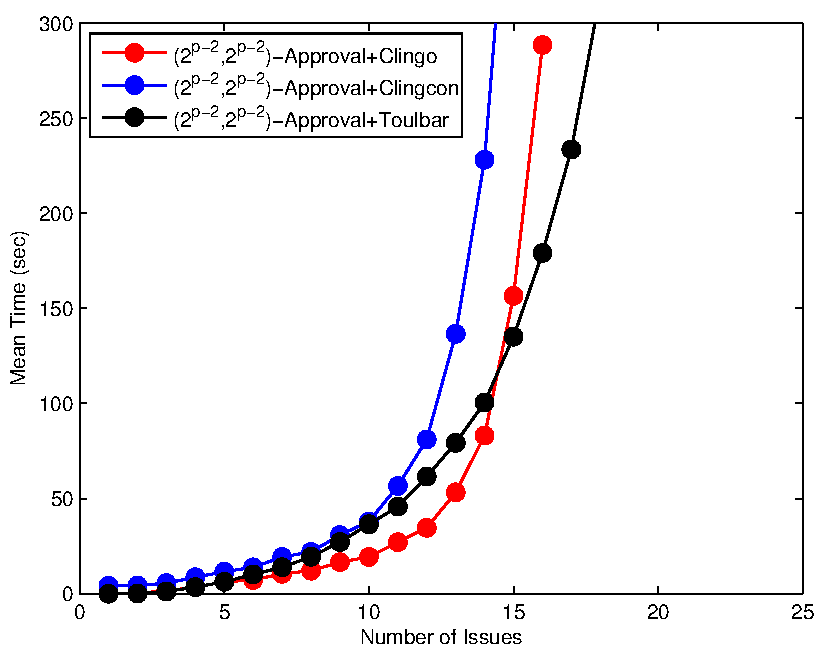
\includegraphics[width=0.95\textwidth]{figs/LPTrees/win/2kAppFVSCICP.pdf}
			\caption{Fixed \#votes (1000)}
		\end{subfigure}
		\caption{Solving the winner problem}
	\end{figure}
}

\frameT{Varying $p$ and $n$: Borda}
{
	\begin{figure}
		\centering
    \begin{subfigure}[b]{0.45\textwidth}
			\centering
			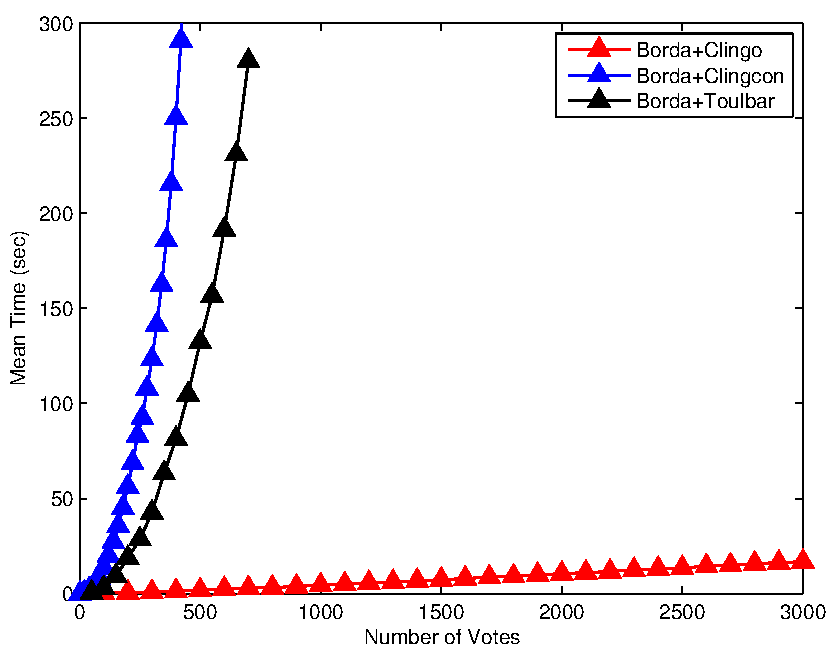
\includegraphics[width=0.95\textwidth]{figs/LPTrees/win/bordaFISCICP.pdf}
			\caption{Fixed \#attributes (10)}
		\end{subfigure}
    \begin{subfigure}[b]{0.45\textwidth}
			\centering
			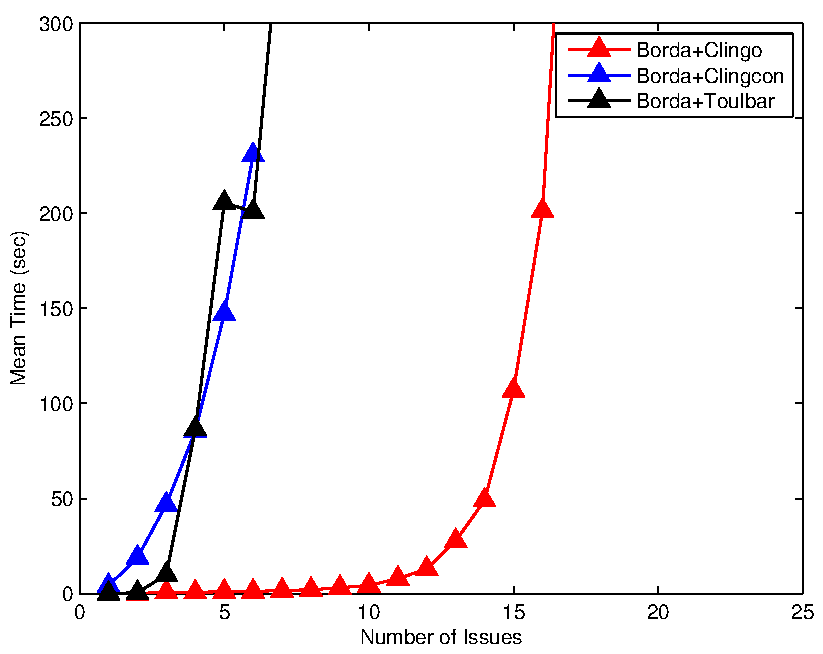
\includegraphics[width=0.95\textwidth]{figs/LPTrees/win/bordaFVSCICP.pdf}
			\caption{Fixed \#votes (1000)}
		\end{subfigure}

		\caption{Solving the winner problem}
	\end{figure}
}

\frameT{Outline}{
  \begin{enumerate}
    {\transparent{0.2} \item The languages of PLP-trees and LP-trees}
    {\transparent{0.2} \item Learning preference models in case of PLP-trees}
    \item Reasoning with preferences:
      \begin{itemize}
        {\transparent{0.2} \item Computing winners and ``strong" candidates when votes are LP-trees}
        \item Application in trip planning
      \end{itemize}
    {\transparent{0.2} \item Future research directions}
  \end{enumerate}
}

\frameT{Personalization in Trip Planning}{
	\begin{enumerate}
		\item Important to incorporate user constraints and preferences into trip
					planning systems.
		\item Collaboration with experts (in AI, planning, optimization, multi-agent systems) at PARC.
		\item Developed a hipergraph-based trip planner that accommodates constraints specified as
					\tit{linear temporal logic} and preferences expressed as \tit{preferential cost function} 
					to compute optimal routes using A*\footcitefull{abs/parc/Liu2}.
		\item Available later for trip planning in the Bay Area, LA, and Denver.
	\end{enumerate}
}

\frameT{Personalization in Trip Planning}{
	\begin{enumerate}
		\item From SJC, to Pier 39, Monday, 9am.
		\item Constraints: never drive a car, and bike for 1 to 2 hours.
		\item Preferences: bike = public (0.25) $>$ wait(2) $>$ walk(3), and 30\$/hr.
	\end{enumerate}

	\vspace{-0.3cm}

	\begin{figure}[ht!]
	  \centering
	    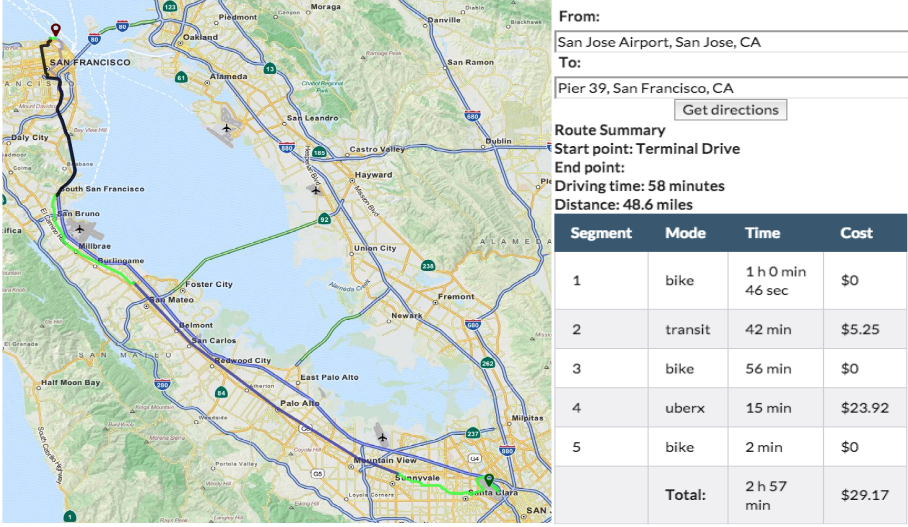
\includegraphics[width=0.7\textwidth]{figs/PARC/route.png}
	\end{figure}
}


\section{Future Research Scenarios}
\frameT{Outline}{
  \begin{enumerate}
    {\transparent{0.2} \item The languages of P-trees, PLP-trees, and LP-trees}
    {\transparent{0.2} \item Learning preference models in case of PLP-trees}
    {\transparent{0.2} \item Reasoning with preferences:
      \begin{itemize}
        \item Computing winners and ``strong" outcomes when votes are LP-trees
        \item Application in trip planning
      \end{itemize}}
    \item Future research directions
  \end{enumerate}
}

\frameT{Data-Driven Preference Engineering}{
	%Goal: preference predicting and feasibility of various preference models.
	\begin{enumerate}
		\item Recommender Systems\footcitefull{adomavicius2005toward}:
			\begin{enumerate}
				\item Collaborative
				\item Content-based
				\item Hybrid
			\end{enumerate}
		\item Machine Learning:
			\begin{enumerate}
				\item Supervised learning (e.g., decision trees, random forests)
				\item Label ranking\footcitefull{hullermeier2008label}
			\end{enumerate}
		\item Preference Elicitation (Human-in-the-Loop):
			\begin{enumerate}
				\item Context-based
			\end{enumerate}
		\item Preference Learning:
			\begin{enumerate}
				\item Conditional Preference Networks, Preference Trees
				\item Stochastic Models (e.g., Choquet integral\footcitefull{leroy2011learning}, 
							TOPSIS-like models\footcitefull{agarwal2014preference})
			\end{enumerate}
	\end{enumerate}
}

\frameT{Preference Reasoning and Applications}{
	%Goal: personalized optimization and collaborative decision making.
	%Goal: exploring collaboration possibilities
	%with experts in other fields.

	\begin{enumerate}
		\item Social Choice and Welfare\footcitefull{arrow2010handbook}:
			\begin{enumerate}
				\item Voting
				\item Fair devision
				\item Strategyproof Social Choice
			\end{enumerate}
		\item Automated Planning and Scheduling:
			\begin{enumerate}
				\item Travel scheduling
				\item Manufacturing
				\item Traffic control
			\end{enumerate}
		\item Computer Vision and Image Processing:
			\begin{enumerate}
				\item Image retrieval
				\item Image and video understanding
			\end{enumerate}
	\end{enumerate}
}

%\frameT{Preference Applications}{
%	Goal: exploring possibilities of collaboration with experts in other areas.
%
%	\begin{enumerate}
%		\item Automated Planning and Scheduling:
%			\begin{enumerate}
%				\item Travel scheduling
%				\item Manufacturing
%				\item Traffic control
%			\end{enumerate}
%		\item Computer Vision and Image Processing:
%			\begin{enumerate}
%				\item Image retrieval
%				\item Image and video understanding
%			\end{enumerate}
%	\end{enumerate}
%}



\section{Conclusion}
%\begin{frame}[allowframebreaks]
%\frametitle{References}
%    \bibliographystyle{abbrv}
%    \bibliography{research}
%\end{frame}
%
\frameT{Questions?}{
	\begin{center}
		Thank you!
	\end{center}
}



\end{document}
